\RequirePackage{tikz}
% Opcje klasy 'iithesis' opisane sa w komentarzach w pliku klasy. Za ich pomoca
% ustawia sie przede wszystkim jezyk i rodzaj (lic/inz/mgr) pracy, oraz czy na
% drugiej stronie pracy ma byc skladany wzor oswiadczenia o autorskim wykonaniu.
\documentclass[english,shortabstract,mgr]{iithesis}

\usepackage[utf8]{inputenc}
\usepackage{ulem}
\usepackage{amsthm}
\usepackage{subcaption}
\usepackage{cite}
\usepackage{float}
\usepackage{multicol}
\usepackage{array}
\usepackage{tabularx}

\usetikzlibrary{shapes.multipart}
\usetikzlibrary{decorations.text}
\usetikzlibrary{automata}


%%%%% DANE DO STRONY TYTUŁOWEJ
% Niezaleznie od jezyka pracy wybranego w opcjach klasy, tytul i streszczenie
% pracy nalezy podac zarowno w jezyku polskim, jak i angielskim.
% Pamietaj o madrym (zgodnym z logicznym rozbiorem zdania oraz estetyka) recznym
% zlamaniu wierszy w temacie pracy, zwlaszcza tego w jezyku pracy. Uzyj do tego
% polecenia \fmlinebreak.
\polishtitle    {Tłumaczenie współczesnego języka programowania\fmlinebreak do Maszyny Minsky'ego}
\englishtitle   {Modern programming language translation to the theoretical model of Minsky Machine (Counter Machine)}
\polishabstract {
Maszyna Mińskiego, zdefiniowana jako skończony zbiór stanów i~przejść między nimi, korzystająca
z~dwóch liczników jako pamięci oraz osobnych liczników odpowiadających za wejście/wyjście, ma
taką samą siłę wyrazu co współczesne języki programowania. To jest znany już fakt, bardziej
popularny w~wersji z Maszyną Turinga. Oznacza to, że dowolny współczesny program da się
przetłumaczyć na teoretyczny model Maszyny Mińskiego.

Moim celem jest zatem zbudowanie automatycznego narzędzia tłumaczącego współczesny język
programowania (Brainfuck) do Maszyny Mińskiego z dwoma licznikami. Tym samym narzędziem
można również przetłumaczyć dany kod źródłowy do Maszyny Mińskiego z czterema
licznikami oraz automatu z dwoma stosami, jak również uruchomić program napisany
w dowolnym z tych języków.
}
\englishabstract{
A Counter Machine, a machine with finite state set, two counters and input/output counters, is~able
to perform any computations done by~modern programming languages. This is theorem
means that anything written in a~modern
programming language can be translated into the~theoretical model of Counter Machine.

I build a tool for automatic translation from a~modern programming language (Brainfuck)
to a~Counter Machine with two counters. The tool can also produce codes for
Counter Machines with four counters, pushdown automata with two stacks as well
as execute a code written in any of these languages.
}
% w pracach wielu autorow nazwiska mozna oddzielic poleceniem \and
\author         {Jadwiga Pokorska}
% w przypadku kilku promotorow, lub koniecznosci podania ich afiliacji, linie
% w ponizszym poleceniu mozna zlamac poleceniem \fmlinebreak
\advisor        {dr Jakub Michaliszyn}
%\date          {}                     % Data zlozenia pracy
% Dane do oswiadczenia o autorskim wykonaniu
\transcriptnum {247906}                     % Numer indeksu
\advisorgen    {dr Jakuba Michaliszyna} % Nazwisko promotora w dopelniaczu
%%%%%

%%%%% WLASNE DODATKOWE PAKIETY
%
%\usepackage{graphicx,listings,amsmath,amssymb,amsthm,amsfonts,tikz}
%
%%%%% WŁASNE DEFINICJE I POLECENIA
%
%\theoremstyle{definition} \newtheorem{definition}{Definition}[chapter]
%\theoremstyle{remark} \newtheorem{remark}[definition]{Observation}
%\theoremstyle{plain} \newtheorem{theorem}[definition]{Theorem}
%\theoremstyle{plain} \newtheorem{lemma}[definition]{Lemma}
%\renewcommand \qedsymbol {\ensuremath{\square}}
% ...
%%%%%

%\usepackage{todonotes}

\newcommand{\todo}[1]{\textbf{TODO:} #1}
\newtheorem*{hypothesis}{Hypothesis}

\begin{document}

\newcolumntype{L}[1]{>{\raggedright\arraybackslash}p{#1}}
\newcolumntype{C}[1]{>{\centering\arraybackslash}p{#1}}
\newcolumntype{R}[1]{>{\raggedleft\arraybackslash}p{#1}}

%%%%% POCZĄTEK ZASADNICZEGO TEKSTU PRACY

\chapter{Introduction}

\section{Turing Machine}

Modern computers and their abilities are complex and depend on many different factors
to~perform given computations, like processor technology, software optimizations within given
processor model, input/output communication protocols and many others. This is why when we want
to~state or prove anything about the behaviour of computer programs, we need a~common
language and~general theoretical model representing any type of ``computer''.

The model is known since 1936 \cite{turing1937computable} when Alan Turing proposed an abstract system
called \textbf{Turing Machine}
to represent a~machine that is able to~execute any computations expressible in~terms of a computer program.
It has all advantages and~disadvantages which belong to~modern programs, i.e., it~is possible
to create a~program which will never stop or~consume an infinite amount of memory. The model does not allow
to~solve all the problems -- it~has the~same limitations in~sense of~creating algorithms
like a~regular computer.

Turing Machine is~a~finite description of~an~algorithm. To perform calculations it uses
a~potentially infinite tape as~its memory -- we have some amount of~tape at~the beginning,
but~we may extend this tape (glue additional tape cells) to~the right end if necessary.
All cells are either blank or~contain a~single letter -- when a~machine starts its
work, it has access to three different tapes: \textit{an input tape}, \textit{an output tape} and
a tape for calculations.
\textit{An input tape} is read-only and it provides symbols one by one until the~end of an~input word
(we cannot perform any direct moves on that tape). Similarly, \textit{an output tape} is write-only, and
when a~machine finishes its work there is an output word written (if any is needed). Using its regular
tape for computations a~machine can do anything: write, read, move and extend the~tape.
After a~machine finishes (if it finishes at all) it can either \textit{accept}
or~\textit{reject} the original input word and there may be an~output word written on the output tape
(for simplicity it is usually assumed that there is no output word).

As~an~example, we can construct a~Turing Machine recognizing all binary palindromes of~even length,
formally defined as a~set $A = \{ ww^R : w \in \{0,1\}^* \}$ (where $w^R$ is the reversed word $w$).
Because we need to use finite description, we say that the~machine should read the whole input word
from the~input tape, store it on its computations tape and move to the~beginning of its tape.
Then the~machine should check the~first letter $a_1$ with the~last one $a_n$ -- if these cells
contain different letters then the~machine should immediately reject the whole word,
otherwise, it should mark both $a_1$ and $a_n$ as checked (i.e. write $\#$ symbol in~their cells)
and~continue with $a_2$ and~$a_{n-1}$. In~the~end, we should have a~tape full of $\#$s and~the~machine
should accept the given word. If there is just one unchanged cell left, then the original word was a~palindrome
of~odd length and~we should reject it.

For the sake of simplicity, we assume we do not have the~output tape -- a~machine may either accept or reject
an~input word written on the~input tape. \textbf{A Turing Machine} is a~$6$-tuple
$(Q,\Sigma,\Gamma,\delta,q_0,P)$ where:
\begin{itemize}
  \item $Q$ is~a~finite set of~states the~machine can be within,
  \item $\Sigma$ is~a~finite input alphabet (does not contain blank),
  \item $\Gamma$ is~a~finite tape alphabet and~$\Sigma \subset \Gamma$,
  \item $\delta: Q \times \Gamma \times \left( \Sigma \cup \{\perp\} \right)
      \rightarrow Q \times \Gamma \times \{L,R\} \times \{-,R\}$  is~a~finite
      transition function, $L$ and~$R$ mean the~machine should move one cell
      left or~right respectively,
  \item $q_0$ is~the~initial state the~machine starts within,
  \item $P$ is~a~finite set of~accepting states.
\end{itemize}

\textbf{Configuration} of~a~Turing Machine is a~triple ($w$, $q$, $k$), where:
\begin{itemize}
  \item $w \in \Gamma^*$ is a~word written on~the~computations tape,
  \item $q$ is a~state the~machine is~currently within,
  \item $k$ is a~cell number the~machine is currently looking at.
\end{itemize}

Having a~configuration, we can precisely say what is the~program execution progress.
One configuration is~a~precise step of~computation, so a~sequence of~configurations (where
each consecutive pair obeys $\delta$) is called
a~\textbf{run} of~a~Turing Machine. This sequence may be finite or~infinite in the~same way as
a~program may loop forever or~finish within some number of~steps. Each such run is not extendable
(there is no $\delta$-travel from the very last state). It begins with
a~configuration, where some word $w$ is~an~input, $k = 0$ which is the~leftmost cell on~the~tape
and~$q = q_0$ which is an initial state defined in~the~description of~the~given machine. If~a~run is
finite and~ends with a~configuration ($w_n$, $q_n$, $k_n$) then we say the~input word to~be
\textit{accepted} if $q_n \in P$ ($q_n$ is one of accepting states) and \textit{rejected} otherwise.

\section{Church-Turing thesis and Turing-completeness}

Computers are used to perform calculations for us. We want them to~execute some
procedures or~to~perform some process and~we call it an~\textit{algorithm} in~its intuitive meaning.
A~good example could be~a~mathematical problem of~generating prime numbers -- it~is fairly simple
to~think of~a~method of~generating prime numbers by checking larger and~larger numbers and~checking
their all possible divisors. We~are able to~precisely say how this algorithm looks like and~if
we think for a~while we would probably be able to~express it in terms of Turing Machines. This
is a consequence of the \textbf{Church-Turing thesis} (see Chapter Church-Turing Thesis of \cite{sipser2012ChurchTuring}):

\textbf{Thesis.} \textit{The intuitive definition of~any~algorithm a~human/computer can follow is~equivalent
to~some description of~a~Turing Machine.}

This thesis allows us to~think about defining algorithms in an intuitive way while still staying
within the~world of~Turing Machine programs.

It~turns out that when designing any~modern algorithms, we use~the same way of the intuitive description
of~a~procedure and~then we~are converting it~into \textit{implementation}, which is~a~representation
of the given algorithm using a~modern programming language. From the thesis, we~claim that
it~would be~possible to~express it~as~a~Turing Machine (but it would probably require lots of~thought).

To~avoid~a~painful process of~expressing algorithms in~an~unhandy theoretical model, we~employ
the~concept of~\textbf{Turing-completeness}. All popular modern programming languages are proven
to~be Turing-complete, which means that we are able to~implement an algorithm in~such
language if and only if there exists some equivalent Turing Machine description.

\section{Counter Machine}

We have one theoretical model so far -- a Turing Machine -- which has the~same power of~expression
as~modern languages. It turns out there are many other theoretical models
equivalent to Turing Machines (so~to~modern languages as~well). One of~such alternatives
is~\textbf{Counter Machine} (sometimes called \textbf{Minsky Machine}) \cite{minsky_67},
which is~really basic in~its construction.

Similarly to~Turing Machine, Counter Machine has~a~finite description -- a finite set of~states $Q$
and~a~transition function $\delta$ defining when the~machine may move from one state to~another.
Instead of~an~infinite tape, there is a fixed number of counters -- each counter works like a~glass of~coins,
the~machine may put a~coin (or~few coins) into the~glass, check whether the~glass is~empty
or~take out a~coin (only one and~only if the glass is not empty). Each counter is a~non-negative
integer, but the~machine is~not allowed to~explicitly check its value, it~just receives boolean
information if it is equal to zero.

There are a few alternative models -- if~we~allow the~machine to~use at~least two counters,
then we get a~model equivalent to Turing Machine. According to~this fact, we~can
choose how many counters it~is convenient to~use. The~only exception is~Counter Machine with
one counter which is~not able to~express everything a~Two Counter Machine can. As~an~argument,
we may say that the halting problem for One Counter Machine is~decidable -- it is possible to~check
in~polynomial time whether a given description of One Counter Machine will loop forever or~not.
Of~course, the halting problem for Two Counter Machine is proven to~be not decidable. \cite{minsky_67}

\section {Two stack pushdown automaton (two stack PDA)}

Similarly to~a~Counter Machine, finite description of a~two stack pushdown automaton
(PDA) contains a~number of~states and~transition function $\delta$,
but~counters are replaced with two stacks
(see Chapter Context-Free Languages, Pushdown Automata of \cite{sipser2012ChurchTuring}).
These two stacks use stack alphabet $\Gamma$ and the~automaton may change their state
by~pushing zero or~more symbols at the~top or~by removing \textbf{exactly one} symbol from
the~top.

In practice, the~implementation assumes that a~single transition \textbf{always} takes
a~symbol from each stack and after transitioning to a~new state pushes some symbols
(maybe the~original ones) to each stack.

Each stack has a~special symbol $\perp$ at the~bottom that determines if the~stack is
empty. Additionally, it is not allowed to take $\perp$ out from the stack, so~after transitioning
to a~new state, $\perp$ must be pushed back (maybe followed by other symbols) to~the~stack.

Formally, two stack PDA is a~$6$-tuple ($Q$, $\Sigma$, $\Gamma$, $\delta$, $q_0$, $F$) where:
\begin{itemize}
  \item $Q$ is a~finite set of states,
  \item $\Sigma$ is a~finite input alphabet ($\epsilon \in \Sigma$),
  \item $\Gamma$ is a~finite stack alphabet ($\perp \in \Gamma$),
  \item $\delta: Q \times \Sigma \times \Gamma \times \Gamma \rightarrow
      Q \times \Gamma^* \times \Gamma^*$ is~a~finite transition function,
  \item $q_0$ is the initial state of the~PDA,
  \item $F$ is a~finite set of accepting states which.
\end{itemize}

Each transition specifies when it may be applied by providing a~quadruple
$(q, a, s, t) \in (Q, \Sigma, \Gamma, \Gamma)$. It means that the input symbol is $a$,
the~left stack has symbol $s$ and the~right stack symbol $t$ at the~top. In practice, there
might be multiple transitions matching the current state, so it is assumed that only the first
defined is applied.

\section{Brainfuck}

A~Counter Machine is~a~minimalistic model of~Turing-complete computations in the same way as
\textbf{Brainfuck} \cite{brainfuckWiki} is a~minimalistic (only eight instructions) programming
language which recalls
the~definition of~Turing Machine -- a program operates on~a~tape containing numbers, it~is possible
to~explicitly read and~change values in~cells. A~program operates on~a~data pointer which
points to~the~current focus cell, so it~is able to~move left or right to the desired cell. The~main difference
between Turing Machine and~Brainfuck is the representation of the source code.
It does not matter what is the order of transitions for Turing Machine, but it
is critical to know what is the order of instructions in Brainfuck.

Usually, Brainfuck implementations assume that tape length is~around $30\,000$ cells, which
is~enough in~most cases. If~we want to~prove Turing-completeness though, this tape
needs to~be potentially infinite. Of course, no~modern machine is~equipped with infinite memory,
but we are able to~extend it (by installing additional hardware), so~this factor is~omitted
when proving Turing-completeness. It is not a~problem in~this thesis at~all since
the~main goal is to~show that anything written in a modern programming language is~possible
to~automatically translate into the theoretical model.

\section {Purpose of this thesis}

This~thesis is a~proof of the theoretical concept based on~Church-Turing thesis -- any~algorithm
or~mathematical method we~are able to~come up with (as~long as it is expressible in any programming
language) is possible to~execute on~the~most basic theoretical model which is a~Counter Machine.

The implementation (\hspace{1sp}\cite{github}) translates Brainfuck into Counter Machine model and~consists of~a~few separate parts
which are separate translations between more and more basic theoretical models.
It is possible to access any transitional program created during the~process.

The~plan of translation includes the following:

\begin{center}
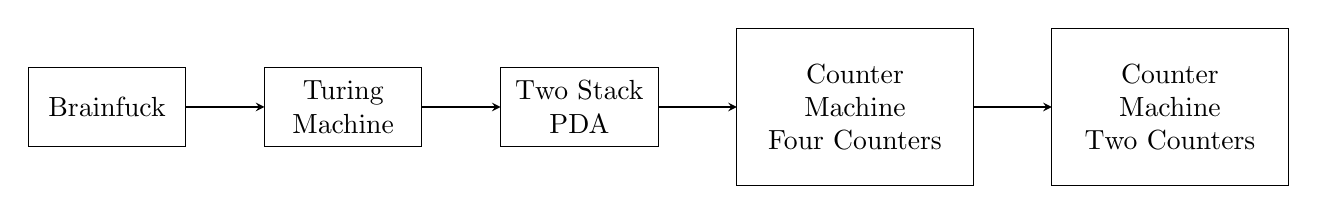
\begin{tikzpicture}
  \draw (0,0) rectangle (2,1) node[pos=.5] {Brainfuck};
  \draw (3,0) rectangle (5,1) node[pos=.5, text width=2cm, align=center] {Turing Machine};
  \draw (6,0) rectangle (8,1) node[pos=.5, text width=2cm, align=center] {Two Stack PDA};
  \draw (9,-0.5) rectangle (12,1.5) node[pos=.5, text width=2.5cm, align=center] {Counter Machine \\ Four Counters};
  \draw (13,-0.5) rectangle (16,1.5) node[pos=.5, text width=2.5cm, align=center] {Counter Machine \\ Two Counters};
  \draw [->, >=stealth] (2,0.5) -- (3,0.5);
  \draw [->, >=stealth] (5,0.5) -- (6,0.5);
  \draw [->, >=stealth] (8,0.5) -- (9,0.5);
  \draw [->, >=stealth] (12,0.5) -- (13,0.5);
\end{tikzpicture}
\end{center}

Any two consecutive models have an automatic translation so we may want to~start with any program written
in Brainfuck, Turing Machine, two stack PDA or a Four Counter Machine and receive an~equivalent Two Counter Machine.
Similarly, we may stop at any point of~translations, so it is possible to generate an equivalent program
in the two stack PDA model from a~program written in the Turing Machine model.

It is worth to mention that there are translators from C to Brainfuck that can
be combined with my work in order to obtain a translation from C to Two Counter
Machine.

This paper is organized as follows: Section 2 contains the exact specification
of all the~models used in translations.
It contains descriptions of how to write source code in each model. Section 3
explains how we approach each separate translation -- the general algorithm
to~move from the~source code in one model
to the~source code in the~next one. Section 4 contains technical details about
the~implementation -- which tools
were chosen for~this project and how to use the~prepared code. It also
discusses the encountered problems and presents
a~summary of the received results. In Section 5, we discuss the~outcome
of the~whole work, what could be extended in the~future
and what could be done better with the~current knowledge.


\chapter {Preliminaries}

\section {Brainfuck}

Brainfuck is a programming language with only eight statements. Execution
of~any program is done using a~finite sequence of~memory cells. Statements
operate on~these cells using a~data pointer --- initially, the pointer is set
on the~leftmost cell in the sequence.

Statements:
\begin{itemize}
  \item \texttt{>} moves the data pointer one cell to the right,
  \item \texttt{<} moves the data pointer one cell to the left,
  \item \texttt{+} increase by one the value held in the cell under the data pointer,
  \item \texttt{-} decrease by one the value held in the cell under the data pointer,
  \item \texttt{.} print to stdout the~character that is under the~data pointer,
  \item \texttt{,} read from stdin a~character and write it to the cell under the data pointer,
  \item \texttt{$[$} beginning of a loop with condition checking whether value under
      the~data pointer is zero. If it is, then execution jumps to the matching $]$,
  \item \texttt{$]$} closing symbol of a loop --- execution jumps to the~beginning of the~loop
      (matching $[$) and then check for zero value under the data pointer is performed.
\end{itemize}

It is allowed to use any other characters within the code, but anything else than the $8$
listed above are ignored --- it is useful for creating comments in the code.

An example code printing ``Hello World!'' (source: \href{https://pl.wikipedia.org/wiki/Brainfuck#Przyk%C5%82ady}{Wikipedia}):
\begin{verbatim}
++++++++++
[
>+++++++>++++++++++>+++>+<<<<-
] We set up the values in a few cells for future use.
>++.               prints 'H'
>+.                prints 'e'
+++++++.           prints 'l'
.                  prints 'l'
+++.               prints 'o'
>++.               prints space
<<+++++++++++++++. prints 'W'
>.                 prints 'o'
+++.               prints 'r'
------.            prints 'l'
--------.          prints 'd'
>+.                prints '!'
>.                 prints newline character
\end{verbatim}

\section {Turing Machine} \label{turing_machine}

\subsection {Instructions}

A~Turing Machine consists of a finite number of states, transition relation
and~a~potentially infinite tape, on~which it is able to~write and~read symbols.
It has no code sequence, a program is a~set of transitions and~a~definition
of~an~initial state. There is a special final state \texttt{END} that does not need
to~be defined to~be used.

There is a~predefined set of symbols used on the tape which is whole ASCII character set
extended with the same amount of additional (non-ASCII) symbols. Regular
ASCII characters have 7 bits (numbers 0-127), so tape symbols have 8 bits
allowing to hold regular ASCII and special characters (numbers 128-255).

        There are few special definitions (it is using regular ASCII, so
these characters may cause unexpected behaviour if used in Brainfuck's
code logic).

\begin{itemize}
  \item \texttt{BLANK} which represents empty field on the tape,
  \item \texttt{*} (\texttt{ALL}) defines all characters (both ASCII and special),
  \item \texttt{\#} (\texttt{NOTHING}) means ``no character'' which is used to say
                   that we do not want to write anything on tape during
                   this state change,
          \item \texttt{\&} (\texttt{NON\_ZERO}) defines all characters except zero,
          \item \texttt{0} (\texttt{ZERO}) represents zero that is used for conditional jumps
           (jump zero),
          \item \texttt{>} (\texttt{NEXT\_CHAR}) allows writing the next character
                   (increased by one) on the~tape i.e. writes \texttt{g}
                   if on the tape was \texttt{f},
  \item \texttt{<} (\texttt{PREV\_CHAR}) similarly as above but writes the previous character,
                   i.e. writes \texttt{e} when seen \texttt{f}.
\end{itemize}

Defining the initial state:
\begin{verbatim}
START: state_name
\end{verbatim}

Each transition looks as follows:
\begin{verbatim}
state_name symbol -> target_state head_move symbol_to_write
\end{verbatim}

\texttt{symbol} is an~ASCII character including special definitions (currently
all special definitions use regular ASCII so that it is easy to see
in a~standard text file).

\texttt{head move} is one of \texttt{L}, \texttt{R} or \texttt{-} which
steer the head to go left, right or stay in place, respectively.

\texttt{symbol to write} is any (currently ASCII) symbol. Writing any symbol
from special definitions will cause undefined behaviour of~the machine. The only symbol
from special definitions that is allowed to appear as \texttt{symbol\_to\_write}
is \texttt{\#} (NOTHING) meaning that symbol on the tape should not change.

\subsection {Extensions of the theoretical model}

Standard input/output handling is done by allowing to read or write a~single
ASCII character from/to stdin/stdout. It is possible to~add additional
reading or~writing instruction before moving the~head. It is done by modifying
the~change symbol \texttt{->} in the~transition definition.
\begin{itemize}
  \item Reading is done with \texttt{->*}, i.e., \texttt{state1 A ->* state2 R NOTHING},
        which means ``when seen the~symbol \texttt{A} in state \texttt{state1}, read
        from stdin one character, overwrite \texttt{A} to the~read value and move
        head one field right''.
  \item Writing is done similarly with \texttt{->\^},
        i.e., \texttt{state1 A ->\^\ state2 R NOTHING}, which will print the~symbol
        \texttt{A} on stdout and move the~head to the~right.
\end{itemize}

\subsection{Example} \label{turing_machine_example}

Below is a~program that reads a~letter from stdin, writes this letter into
stdout and if the~written letter was \texttt{B} or \texttt{b} then prints
\texttt{.} at the end as well, otherwise finishes.

\begin{verbatim}
START: s1
s1 ALL ->* s2 - NOTHING
s2 ALL ->^ s3 - NEXT_CHAR
s3 ALL -> s4 - NOTHING
s4 b ->^ s5 R NOTHING
s4 B ->^ s5 R NOTHING
s5 ALL -> s6 - .
s6 ALL ->^ s7 - NOTHING
s7 ALL -> END - NOTHING
\end{verbatim}

Note: If there is no transition defined for the given configuration
(nothing matches), then it is assumed that the~machine gets to the~\texttt{END} state.
Because of this, in the above example, last instruction is not necessary.

\section {Two Stack Pushdown Automaton}

A~Two Stack Pushdown Automaton consists of two stacks, an~input tape and~a~definition
of~states and transitions between them. Each transition looks as follows:
\begin{verbatim}
state_name left_pattern right_pattern ->
    target_state left_stack_items right_stack_items
\end{verbatim}

Explanation:
\begin{itemize}
  \item \texttt{left\_pattern} is a~symbol or a~pattern that should be matched
      for the symbol at the top of the left stack,
  \item \texttt{right\_pattern} is the same as above but for the right stack,
  \item \texttt{left\_stack\_items} is the list of items that should be pushed
      to the~left stack before moving to \texttt{target\_state}. It might be
      a~single letter \texttt{"a"}, a~sequence of letters \texttt{"abc"}
      or~a~sequence of~letters and~references, i.e., \texttt{("a" + ORIG\_LEFT + "b")}
      where \texttt{ORIG\_LEFT} means the letter we read from the~left stack (the one matched
      in \texttt{left\_pattern}). Note: If \texttt{+} is used, it is required to put
      the~whole sequence in parenthesis,
  \item \texttt{right\_stack\_items} is the same as above, but for items to be pushed into
      the right stack.
\end{itemize}

Special references and definitions in transitions:
\begin{itemize}
  \item \texttt{ORIG\_LEFT} is the letter taken from the left stack,
  \item \texttt{ORIG\_RIGHT} is the letter taken from the right stack,
  \item \texttt{INPUT\_CHAR} is the letter taken from the input tape
      (only in the~input transition type - see the section below),
  \item \texttt{NOTHING} may be used as \texttt{left\_stack\_items} or \texttt{right\_stack\_items}
      and means that nothing is pushed into the left/right stack,
  \item \texttt{END} is a special state name into which the transition is made if no other transition is specified,
  \item \texttt{\$} is the symbol of the stack bottom.
\end{itemize}

\subsection {Extensions of the theoretical model}

Input/Output handling is done similarly to a~Turing Machine: we change \texttt{->} in transition
to \texttt{->*} or \texttt{->\^}.

When defining input transition, it is allowed to use \texttt{INPUT\_CHAR} in any items
to be pushed into the left/right stack. Here is an~example that takes a~character from input
tape and pushes it into the~left stack (and ignores symbols taken from both stacks).
\begin{verbatim}
state1 ALL ALL ->* state2 INPUT_CHAR NOTHING
\end{verbatim}

When defining output transition we \textbf{must} specify what character is printed
with adding \texttt{Output: <letter>} at the very back of the~transition definition.
An~example that prints the~letter taken from the~left stack (and ignores what was
taken from the~right stack):
\begin{verbatim}
state1 ALL ALL ->^ state2 NOTHING NOTHING Output: ORIG_LEFT
\end{verbatim}
An~example that prints the~letter ``a'' (and ignores what was taken from the~stacks):
\begin{verbatim}
state1 ALL ALL ->^ state2 NOTHING NOTHING Output: "a"
\end{verbatim}

\textbf{Important note:} Order of defining transition matters. If patterns do not match
a~distinct set of letters, then the transition that appeared first is applied.

\subsection{Example}

An~example (equivalent to the example from Turing Machine):
\begin{verbatim}
START: init_state
init_state $ $ -> s1 BLANK NOTHING
s1 ALL ALL ->* s2 INPUT_CHAR ORIG_RIGHT
s2 ALL ALL ->^ s3 ORIG_LEFT ORIG_RIGHT Output: ORIG_LEFT
s3 b $ -> s4 (ORIG_LEFT + BLANK) $
s3 b ALL -> s4 (ORIG_LEFT + ORIG_RIGHT) NOTHING
s3 B $ -> s4 (ORIG_LEFT + BLANK) $
s3 B ALL -> s4 (ORIG_LEFT + ORIG_RIGHT) NOTHING
s4 ALL ALL -> s5 "." ORIG_RIGHT
s5 ALL ALL ->^ s6 ORIG_LEFT ORIG_RIGHT Output: ORIG_LEFT
s6 ALL ALL -> END ORIG_LEFT ORIG_RIGHT
\end{verbatim}

\section {Counter Machine (four counters)}

A~Four Counter Machine consists of four counters each holding non-negative integer,
a~finite number of states and~transitions between them. Each transition
looks as follows:

\begin{verbatim}
state_name (pattern pattern pattern pattern) ->
    target_state (number number number number)
\end{verbatim}
%
where:
\begin{itemize}
  \item \texttt{state\_name} is the state in which the Counter Machine needs to be
      within for this transition to be applied,
  \item \texttt{pattern} is one of values \texttt{0}, \texttt{1} or \texttt{\_}.
      \texttt{0} means we expect the~empty counter, \texttt{1} means we expect an~non-empty
      counter and \texttt{\_} means that this counter state does not matter, so
      this transition should be applied regardless of this counter's value,
  \item \texttt{target\_state} is the state in which machine will be after
      applying the transition,
  \item \texttt{number} is an~integer from the~range \texttt{[-1, MAX\_INT]} specifying
      what should be added to a given counter - it is allowed to decrease a counter
      by one only, but it is possible to increase it by any number that can be stored
      in a~regular integer type.
\end{itemize}

\textbf{Note:} If there are many transitions that may be applied in a~given state
matching all the counters, \textbf{the first one} is applied. It means that the order
of defining transitions matters.

It is required to give an~initial state of the machine with the following statement:
\begin{verbatim}
START: state_name
\end{verbatim}

\subsection {Extensions of the theoretical model}

The~Input/Output operations fit in the schema of using counters - input and output
are additional counters which transitions may be used in a~similar way as counters are used.

An~input transition is defined as follows:
\begin{verbatim}
state_name (counters) input pattern ->*
    target_state (numbers) input_operation
\end{verbatim}
%
where:
\begin{itemize}
  \item \texttt{input\_pattern} is one of \texttt{0}, \texttt{1} or \texttt{\_}
      (same as the counter pattern) and specifies what should be the state
      of input counter for this transition to be applied,
  \item \texttt{input\_operation} specifies what action should be performed
      on the~input counter and is one of \texttt{LOAD}, \texttt{-1} or \texttt{NOOP}
      meaning respectively loading a~character from stdin into the input counter,
      decrease input counter by one, and leaving input counter untouched.
\end{itemize}

This transition reads from stdin into the input counter:
\begin{verbatim}
state1 (_ _ _ _) _ ->* state2 (0 0 0 0) LOAD
\end{verbatim}

These transitions read the~value from the~input counter and store it in the first counter:
\begin{verbatim}
state1 (_ _ _ _) 1 ->* state1 (1 0 0 0) -1
state1 (_ _ _ _) 0 ->* state2 (0 0 0 0) NOOP
\end{verbatim}

Note: Any transition may only decrease (or load) the input counter
and it is not allowed to increase its value.

An~output transition is defined as follows:
\begin{verbatim}
state_name (counters) ->^ target_state (numbers) Output: output_operation
\end{verbatim}
%
where \texttt{output\_operation} specifies what should be performed on the~output
counter and may be one of \texttt{FLUSH} or non-negative number, meaning
respectively pushing the~counter to stdout and modifying the~value stored
in the counter by the~given number.

These transitions print character stored in the first counter:
\begin{verbatim}
state1 (1 _ _ _) ->^ state1 (-1 0 0 0) Output: 1
state1 (0 _ _ _) ->^ state2 (0 0 0 0) Output: FLUSH
\end{verbatim}

Note: Any transition may only increase (or flush) the output counter
and is not allowed to decrease its value.

\subsection{Example}

A~code that reads a~character from stdin, doubles its ASCII value and prints
the result is as follows:
\begin{verbatim}
START: s1
s1 (_ _ _ _) _ ->* s2 (0 0 0 0) LOAD
s2 (_ _ _ _) 1 ->* s2 (1 0 0 0) -1
s2 (_ _ _ _) 0 ->* s3 (0 0 0 0) NOOP
s3 (1 _ _ _) -> s3 (-1 2 0 0)
s3 (0 _ _ _) -> s4 (0 0 0 0)
s4 (_ 1 _ _) ->^ s4 (0 -1 0 0) Output: 1
s4 (_ 0 _ _) ->^ END (0 0 0 0) Output: FLUSH
\end{verbatim}

\section {Counter Machine (two counters)}

A~Counter Machine with two counters has the same definition as
a~Counter Machine with four counters, but it is allowed to use only
two counters, so transitions become of the form:

\begin{verbatim}
state_name (pattern pattern) -> target_state (number number)
\end{verbatim}

Input/Output is handled the same way it is handled in a~Counter Machine with four counters.


\chapter{Theoretical underpinnings}

\section {From Brainfuck to Turing Machine}

Brainfuck is very similar to the Turing Machine, so it is relatively easy to build
a~translation. They both have a~tape and both can read and update symbols in any
cell of the~tape. There are two main differences: representation of states and
input/output handling.

\textit{States representation.}
Brainfuck has a~sequence of instructions that need to~be
executed one by~one in the~given order, while Turing Machine has an unordered set
of states and transition function (defining how to move between them). A solution
is to give a~unique name to each instruction and specify transitions between
consecutive instructions. The only exception is a~loop, where depending on
symbol stored in the current cell we perform the transition to one out of two different states.
This is exactly what the Turing Machine model provides -- depending on the~symbol
within the current cell, we apply the appropriate transition.

\textit{Input/Output handling.}
A~Turing Machine can either accept or~reject a~given input, so it is necessary to
extend this theoretical model to allow side-effects like reading the~standard
input and writing to the~standard output. Even though there is a~way to give
an~input word (it should be initially written on the tape), this thesis assumes
that there are a separate source and a separate destination for input/output operations.
It means that at any point we may load a~symbol into the current cell or~send
any symbol (not necessarily the one from the current cell) to the~screen. This
way Brainfuck itself handles input/output as well, which makes the~translation straightforward.

\section {From Turing Machine to two stack PDA}

A~Turing Machine operates on a~tape, while two stack PDA operates on two stacks, so we need
to represent a~tape using two stacks. The idea is well-known: we cut the~tape into
two pieces in a~way that the current cell is at the~top of the~left stack and all
the cells from the~left side are lower in the~left stack and similarly all cells from the~right side
are stored in the~right stack (cell to the right of the~current cell is the top of the~right stack).

The only problem is the~fact that Turing Machine tape is infinite in one direction.
There is an~exact cell that contains the very last non-blank symbol, so we assume the~tape
ends at this symbol to perform our cut. If Turing machine at any point decides to extend
the tape, it needs to first move into a new cell (make this cell top of the~left stack in our PDA),
so at this point, two stack PDA model can simply insert an additional new element to the left
stack performing this extension.

It is clear what are the equivalent operations to the ones a~Turing Machine performs.
For example equivalent operation to updating the current cell is taking one symbol from
the~top of the left stack and push the new symbol in its place. Moving one cell to the~right
is equivalent to taking one symbol from the~top of the~right stack and pushing it
into the~left stack -- if the~right stack is empty then we just push the new blank symbol
to the~left stack.

\section {From two stack PDA to four Counter Machine}

Similarly to the~reduction from Turing Machine to two stack PDA we need to simulate
one memory model with the~other one. In this case, we need to simulate two stacks
with four counters. More precisely, it is enough to show how to simulate one stack
with two counters and then apply the~same idea to both stacks.

A~stack alphabet $\Gamma$ is finite and is of size $N = |\Gamma|$. Each symbol from $\Gamma$ may
be assigned a~unique number starting from $1$ up to $N$ ($0$ is problematic -- it will be
explained later). A~stack is a~sequence of numbers $a = a_0 a_1 a_2 \dots a_{k}$ (where $a_0$
is the~stack top and $a_k = \perp = 0$ is the~stack bottom). We represent such
a~sequence as a~single number in a~numeral system with base $\bar{N} = N+1$:

$$ a_0 \cdot \bar{N}^0 + a_1 \cdot \bar{N}^1 + \dots + a_{k} \cdot \bar{N}^{k}
    = \sum_{i=0}^{k} a_i \cdot \bar{N}^i $$

Our left counter will hold the whole stack as a~single number and our right counter will be used
to perform operations on the~left one. Because of this representation if we had some symbol $a$
with the~value $0$, then we would not distinguish between an~empty stack and the~one containing
a single $a$ (more precisely, $0$ could represent a~stack containing any number of $a$'s
stored on this stack).

We need a~few stack operations (and their equivalent
methods on counters):
\begin{itemize}
  \item \textbf{pop} one symbol from the~top,
  \item \textbf{push} one symbol to the~top,
  \item \textbf{check} what is the~symbol at the~top.
\end{itemize}

To \textbf{pop} one symbol from the~stack we just perform an~integer division by $\bar{N}$ on
the~counter. To~perform this division we decrease the~counter by one at each step and every
$\bar{N}$-th step we increase the~helper counter by one. When the~original counter becomes empty,
then the~helper counter stores the~result of integer division by $\bar{N}$. Now we just
need to copy the~result from helper counter into the~original one. The whole operation shows
Figure \ref{fig:pop_operation}.

\begin{figure}[H]
  \begin{subfigure}[b]{0.4\textwidth}
    \centering
    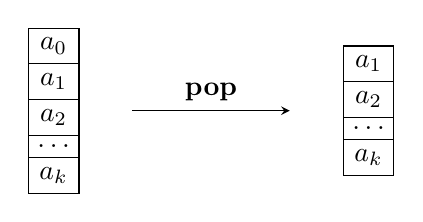
\begin{tikzpicture}[stack/.style={rectangle split, rectangle split parts=#1,draw, anchor=center}]
      \node[stack=5] at (0,0) {
        \nodepart{one}$a_0$
        \nodepart{two}$a_1$
        \nodepart{three}$a_2$
        \nodepart{four}$\dots$
        \nodepart{five}$a_{k}$
      };

      \node[stack=4] at (4,0) {
        \nodepart{one}$a_1$
        \nodepart{two}$a_2$
        \nodepart{three}$\dots$
        \nodepart{four}$a_{k}$
      };

      \draw [->, >=stealth] (1,0) -- (3,0) node [midway, above, sloped] (TextNode) {\textbf{pop}};
    \end{tikzpicture}

    \captionsetup{font=footnotesize}
    \caption{Pop $a_0$ from the top.}

  \end{subfigure}
  \begin{subfigure}[b]{0.6\textwidth}
    \centering
    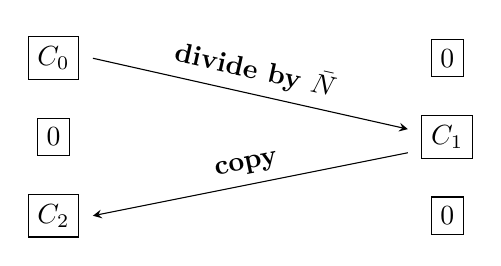
\begin{tikzpicture}[stack/.style={rectangle split, rectangle split parts=#1,draw, anchor=center}]

      \node[stack=1] at (0,2) { \nodepart{one}$C_0$ };
      \node[stack=1] at (5,2) { \nodepart{one}$0$ };

      \node[stack=1] at (0,1) { \nodepart{one}$0$ };
      \node[stack=1] at (5,1) { \nodepart{one}$C_1$ };

      \node[stack=1] at (0,0) { \nodepart{one}$C_2$ };
      \node[stack=1] at (5,0) { \nodepart{one}$0$ };

      \draw [->, >=stealth] (0.5,2) -- (4.5,1.1) node [midway, above, sloped] (TextNode) {\textbf{divide by $\bar{N}$}};
      \draw [->, >=stealth] (4.5,0.8) -- (0.5,0) node [midway, above, sloped] (TextNode) {\textbf{copy}};

    \end{tikzpicture}

    \captionsetup{font=footnotesize}
    \caption{Pop $a_0$ from the~stack encoded in counter $C_0$.}

  \end{subfigure}

  \caption{Stack vs. counter --- the~\textbf{pop} operation.}
  \label{fig:pop_operation}

\end{figure}

To \textbf{push} the~symbol $b$ to the~top of the stack we need to multiply the~counter
by $\bar{N}$ and add the~number $\bar{b}$ corresponding to symbol $b$:
$$ \bar{b} + \bar{N} \cdot
    \Big[ a_0 \cdot \bar{N}^0 + a_1 \cdot \bar{N}^1 + \dots
    + a_{k} \cdot \bar{N}^{k} \Big]
    = \bar{b} + \sum_{i=0}^{k} a_i \cdot \bar{N}^{i+1} $$
Schematic operations to push stack symbol into a~stack represented as a~number are
shown in Figure \ref{fig:push_operation}.

\begin{figure}[H]
  \begin{subfigure}[b]{0.4\textwidth}
    \centering
    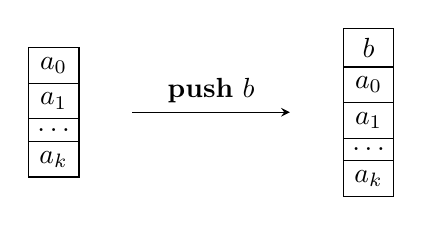
\begin{tikzpicture}[stack/.style={rectangle split, rectangle split parts=#1,draw, anchor=center}]
      \node[stack=4] at (0,0) {
        \nodepart{one}$a_0$
        \nodepart{two}$a_1$
        \nodepart{three}$\dots$
        \nodepart{four}$a_{k}$
      };

      \node[stack=5] at (4,0) {
        \nodepart{one}$b$
        \nodepart{two}$a_0$
        \nodepart{three}$a_1$
        \nodepart{four}$\dots$
        \nodepart{five}$a_{k}$
      };

      \draw [->, >=stealth] (1,0) -- (3,0) node [midway, above, sloped] (TextNode) {\textbf{push} $b$};
    \end{tikzpicture}

    \captionsetup{font=footnotesize}
    \caption{Push $b$ to the top.}

  \end{subfigure}
  \begin{subfigure}[b]{0.6\textwidth}
    \centering
    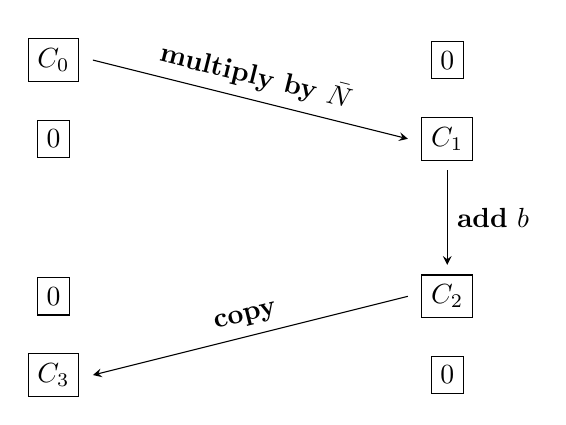
\begin{tikzpicture}[stack/.style={rectangle split, rectangle split parts=#1,draw, anchor=center}]

      \node[stack=1] at (0,4) { \nodepart{one}$C_0$ };
      \node[stack=1] at (5,4) { \nodepart{one}$0$ };

      \node[stack=1] at (0,3) { \nodepart{one}$0$ };
      \node[stack=1] at (5,3) { \nodepart{one}$C_1$ };

      \node[stack=1] at (0,1) { \nodepart{one}$0$ };
      \node[stack=1] at (5,1) { \nodepart{one}$C_2$ };

      \node[stack=1] at (0,0) { \nodepart{one}$C_3$ };
      \node[stack=1] at (5,0) { \nodepart{one}$0$ };

      \draw [->, >=stealth] (0.5,4) -- (4.5,3) node [midway, above, sloped] (TextNode) {\textbf{multiply by $\bar{N}$}};
      \draw [->, >=stealth] (5,2.6) -- (5,1.4) node [midway, right] (TextNode) {\textbf{add} $b$};
      \draw [->, >=stealth] (4.5,1) -- (0.5,0) node [midway, above, sloped] (TextNode) {\textbf{copy}};

    \end{tikzpicture}

    \captionsetup{font=footnotesize}
    \caption{Push $b$ to the~stack encoded in counter $C_0$.}

  \end{subfigure}

  \caption{Stack vs. counter --- the~\textbf{push} operation.}
  \label{fig:push_operation}

\end{figure}


The hardest part is to recognize what is the~top symbol -- the~\textbf{check} operation.
The idea is simple -- we need to calculate the~remainder from the division by $\bar{N}$:
$$ \Bigg( \sum_{i=0}^{k} a_i \cdot \bar{N}^i \Bigg) \ \mathrm{mod} \ \bar{N} = a_0 $$
The only places where we can remember any information are states. This means that we need
to end up within a different state for each remainder -- we call a~state $R_i$ if
the recognized symbol has the~number $i$. Consider an~example alphabet having $9$ symbols -- Figure
\ref{fig:check} shows all states and transitions needed to~recognize it. Each
transition labelled with $0$ is applied only when the counter is empty, similarly
all those labelled with $1$ apply when it is not empty. Additionally, when we move around
the~circle (apply the~transition labelled with $1$), we always decrease the~counter.

\begin{figure}[H]
\centering
\begin{tikzpicture}
\foreach \a in {0,1,...,9}{
  \ifnum\a=0 {
    \node [state,initial] (q0) at (180: 2.5cm) {$q_0$};
  }
  \else{
    \node [state] (q\a) at (-\a*360/10 + 180: 2.5cm) {$q_{\a}$};
  }\fi
}

\foreach \a in {1,2,...,9}{
  \xdef \textplace {right}
  \ifnum\a>4 {\xdef \textplace {left}}\fi
  \ifnum\a=1 {\xdef \textplace {above}}\fi
  \ifnum\a=4 {\xdef \textplace {above}}\fi
  \ifnum\a=5 {\xdef \textplace {above}}\fi
  \ifnum\a=6 {\xdef \textplace {below}}\fi
  \ifnum\a=9 {\xdef \textplace {below}}\fi
  \node [state,accepting] (R\a) at (-\a*360/10 + 180: 5cm) {$R_{\a}$};
  \path[->] (q\a) edge node [\textplace] {0} (R\a);
}

\foreach \a in {0,1,...,9}{
  \xdef \textplace {above}
  \ifnum\a>4 {\xdef \textplace {below}}\fi
  \ifnum\a=0 {\xdef \textplace {left}}\fi
  \ifnum\a=9 {\xdef \textplace {left}}\fi
  \ifnum\a=4 {\xdef \textplace {right}}\fi
  \ifnum\a=5 {\xdef \textplace {right}}\fi
  \path[->] (q\a) edge [bend left=20] node [\textplace] {1} (q\intcalcMod{\a+1}{10});
}
\end{tikzpicture}

\caption{Recognizing a~symbol from an alphabet of size $9$. $R_i$ is the~state with recognized
  symbol $i$, labels on paths define whether the~counter is empty (0) or not (1).}
\label{fig:check}

\end{figure}

When a~counter value decreases to zero, then we move to some state $R_i$ (notice that for
the~correct representations of the~stacks we never get a~remainder equal zero, so we never end within $q_0$).
If we do not want to destroy the~original counter value (which is the~stack representation), we need
to copy it into our counter for computations and after recognizing the~symbol at the~top,
we need to copy it back to the original counter.

\textit{How to put it all together?}

Because all transitions (in any presented model) are independent, we may focus on a~single
transition and when we build a~translation for it, then we can build a~translation for the~whole
program (as long as we keep the~order of transitions).

Each two stack PDA transition \texttt{T} has a~\texttt{state} the~model needs to be within,
an~\texttt{other\_state} to which the~model moves into \textbf{if both stack symbols match
the~patterns}.

\begin{verbatim}
state left_symbol right_symbol -> other_state [...]
\end{verbatim}

We will keep the~state names and build a~new Four Counter Machine model that will operate
on states \texttt{state} and \texttt{other\_state}, but as well as some additional states
in between. To check whether $T$ should be applied, we perform two \textbf{check}
operations. Because both symbols need to match, after recognizing the first symbol
we need to recognize the other one without losing the information about the~first one. This
means that we build a~structure from Figure \ref{fig:check} and in place of each $R_i$ we
paste the same structure for symbols recognition. All unsuccessful paths (symbols not matched)
return to \texttt{state} and successful ones end up within \texttt{other\_state}.

This idea gives O($m^2$) new transitions, where $m$ is the~number of transitions in the two stack PDA
program. If we consider the~input counter (which is yet another input stack), then we get O($m^3$)
transitions that we generate. Fortunately, implementation optimizations make it O($m^2$).

There are still a~few more details to handle:
\begin{itemize}
  \item each applied transition performs a~\textbf{pop} (it always pops a~top element),
  \item transitions may push some items to the stacks (these items may contain symbols that
      were just popped),
  \item a~transition may contain output instruction.
\end{itemize}

Notice that pushing symbols (even a few ones) is easy -- we need to apply \textbf{push} operation
multiple times, no matter if it is a~stack or an~output. It is worth to notice
that building this structure takes O($N$) new states assuming the~number of symbols
to push is constant. The whole transition $T$ takes O($N \cdot m^2$) newly
generated states.

In practice, we want to pop elements together with recognizing them, but now we define the~idea, so
it is enough to say that we perform a~\textbf{pop} after making sure we should apply transition $T$.

\section {From Four Counter Machine to Two Counter Machine}

We discuss how to compress four counters into only two counters. Previously we had
two counters per each stack (from two stack PDA), where one counter was
for the state and the other one was used for calculations. We will do a similar
thing -- we will compress all four counters states into only one counter
(called \textit{general counter}) and use the other one
(called \textit{calculations counter}) for calculations. Here is how we define
the compression:
$$ (A\ B\ C\ D) \rightarrow 2^A \cdot 3^B \cdot 5^C \cdot 7^D$$
where $A$, $B$, $C$ and $D$ are the states of the four counters. Because each
number has a unique factorization using prime numbers (in our case
prime numbers $2$, $3$, $5$ and $7$), we can revert this compression
to get original counters states. It could be any prime numbers,
but for efficiency and simplicity, it is assumed that these are four smallest
prime numbers.

To increase $A$ by some constant $c$, we need
to multiply the general counter by $2^c$, similarly to decrease $A$
(we decrease by one only) then we need to divide by two.

Multiplying by $2^c$ is easy to express in the $2$CM world:
\begin{enumerate}
  \item repeat as long as the general counter is not empty:
  \begin{enumerate}
    \item decrease the general counter by one,
    \item increase the calculation counter by $2^c$,
  \end{enumerate}
  \item once the general counter is empty then copy calculation counter back to general counter.
\end{enumerate}

The translation of a transition:
\begin{verbatim}
s (_ _ _ _) -> next_s (1 0 2 0)
\end{verbatim}
%
will look like this:
\begin{verbatim}
s (_ _) -> s_modify (0 0)
s_modify (1 _) -> s_modify (-1 2)
s_modify (0 _) -> s_recover (0 0)
s_recover (_ 1) -> s_recover (1 -1)
s_recover (_ 0) -> s_modify2 (0 0)

s_modify2 (1 _) -> s_modify2 (-1 25)
s_modify2 (0 _) -> s_recover2 (0 0)
s_recover2 (_ 1) -> s_recover2 (1 -1)
s_recover2 (_ 0) -> next_s
\end{verbatim}


Making division is harder. We will do something similar to recognizing the top
character when translating two stack PDA to $4$CM. For such transitions (recognizing
whether second counter is empty or not):
\begin{verbatim}
s (_ 1 _ _) -> s_1 (0 0 0 0)
s (_ 0 _ _) -> s_0 (0 0 0 0)
\end{verbatim}
%
such a circle is built (end up within \texttt{s\_0} if counter is empty and in \texttt{s\_1} otherwise):

\begin{center}
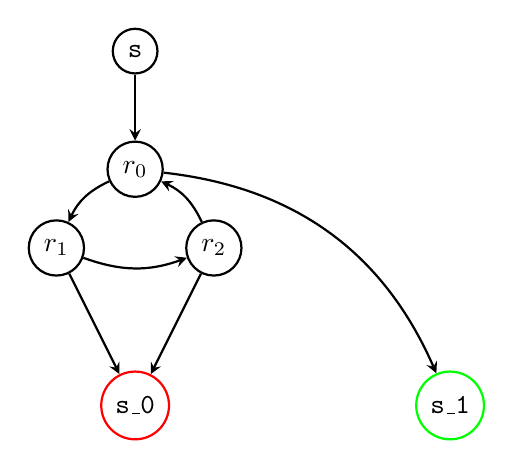
\begin{tikzpicture}
  \node [shape=circle, draw=black, thick] (s) at (0,1.5) {\texttt{s}};
  \node [shape=circle, draw=black, thick] (r0) at (0,0) {$r_0$};
  \node [shape=circle, draw=black, thick] (r1) at (-1,-1) {$r_1$};
  \node [shape=circle, draw=black, thick] (r2) at (1,-1) {$r_2$};

  \node [shape=circle, draw=red, thick] (s1) at (0,-3) {\texttt{s\_0}};
  \node [shape=circle, draw=green, thick] (s0) at (4,-3) {\texttt{s\_1}};


  \path [->,thick,>=stealth] (s) edge (r0);
  \path [->,thick,>=stealth] (r0) edge[bend right=20] (r1);
  \path [->,thick,>=stealth] (r1) edge[bend right=20] (r2);
  \path [->,thick,>=stealth] (r2) edge[bend right=20] (r0);

  \path [->,thick,>=stealth] (r0) edge[bend left=30] (s0);
  \path [->,thick,>=stealth] (r1) edge (s1);
  \path [->,thick,>=stealth] (r2) edge (s1);
\end{tikzpicture}
\end{center}

Additionally just before entering states \texttt{s\_0} and \texttt{s\_1}
we need to move everything from the calculations counter back to general counter.

The picture would be much more complex if the original $4$CM transition
recognized more counters. Fortunately, all the transitions produced by
the automatic translation use at most one counter (for recognition),
so for the purpose of this thesis, such an example is not necessary.

\chapter{Implementation}

\section{Introduction}

The language chosen for the entire project is C++, mainly because of its efficiency. Counter Machine
is a~basic model, so any translated program is expected to be very long. These amounts of information
need to be stored and accessed efficiently, so STL library and its containers like hashing table
and hashing set are used heavily in this project. Sources are available online \cite{github}.

For translation purposes, we need to have access to abstract syntax trees of original programs, which
means that we should be able to parse a~source code. To do so, we use the most common tools
for lexing and parsing in C++, Flex and Bison. We have several translations
between several different models, so at every step (i.e. Turing Machine to two stack PDA) Flex and Bison
are applied to parse a~source code (i.e. in Turing Machine model) and produce abstract syntax tree.
This tree is later used either for evaluation (if we want to execute) or translation to the~next
model in the~pipeline (i.e. two stack PDA).

Most of the translations are pretty straightforward and require only basic tricks like
generating unique state names. The~most interesting one is Two Stack PDA to Four Counter Machine,
which requires putting a large part of a~program logic into appropriate state names, so it is important
to notice the~structure of the~logic to come up with a reasonable translation algorithm.
It turns out that Brainfuck has very specific instructions that allow making optimizations
to the~translation process. These optimizations allowed to generate a shorter
code.

Few examples:
\begin{itemize}
  \item Input is always a~single symbol and it is directly stored within one of the~memory cells,
      which means we do not need to recognize what is read -- we just blindly store it in memory.
      This is the~optimization mentioned earlier -- we may use only O($m^2$) new states to translate
      a~single two stack PDA transition.
  \item Merging all failing paths into one state. As shown in Figure \ref{fig:check},
      we end up in some $R_i$ depending on the recognized symbol.
      Sometimes we are interested in recognizing only one specific symbol
      and want the code to fail (stop the execution) for all the others.
      Int this case all $R_i$'s, except the desired one,
      may be merged into one state (\texttt{END}).
  \item two stack PDA interpreter always recognizes symbols on both stacks
      to check what is the matching transition. This strategy (when translated
      explicitly to $4$CM) results in lots of code (O($m^2$) states generated
      from a single transition). Original Brainfuck's \texttt{+} and \texttt{-}
      does not need both symbols -- it checks the one on the left stack,
      increases it by one and stores it back onto the same (left) stack.
      This means that the right stack may be completely ignored. This will
      result in O($m$) transitions in $4$CM from a single two stack PDA transition.
\end{itemize}


There are also optimizations in the interpreters so that the existing
translated code is executed more efficiently:

\begin{itemize}
\item There is no need to load all the states at the beginning because most probably we will
      not need all of them -- lazy loading allows to add to transition set
      only the transitions that refer to the state that we are currently in.
  \item In $2$CM transitions, we often need to recover the counter's position by
      copying its content to the other counter. Such a transition subtracts
      one and adds one on desired counters, which is a very ineffective copy.
      Such a transition is recognized and the copy is done immediately with
      regular variable assignment in C++.
\end{itemize}



The amount of generated information is very big even for the simplest programs, which is not a surprise.
After analyzing a classical \textit{Hello World!}, it turns out that a~human can
significantly reduce the~required logic. Automatic translation will store single letters
in memory (on a~tape or on a~stack) and then print it out, while we may directly use output
tape/stack/counter. This is caused by the Brainfuck code structure, where the only thing we can do
is modifying the~memory and then output what is within this memory.

The other problematic operation was shifting Brainfuck's tape --- when we shift
by one position on the tape then our stack in Turing Machine (and later languages)
grows by one character. When we remind ourselves what it means to extend a counter by
one character we realise why is it so -- a counter needs to be multiplied by
the~size of the~alphabet and increased by the~character's ASCII number.
This means that each time we shift right we increase our counter 140 times
(which is the alphabet size set within the program) and what is more, next
iterations of a~program need to recognize characters on the top of that
counter with decreasing it by one at a time.

The time of computations starts to be an issue at the very end of the pipeline, namely
when executing a $2$CM program. Because of the structure of the counter translation
(exponential) and the way this (exponential) counter is used, it is really
hard to get any English character. ASCII table contains these characters
at high positions like 65 ('A'), so within our $2$CM's counter it will be represented
as a number $2^{65}$ if it was on the first counter of $4$CM and $3^{65}$ when
it is moved to the second counter of $4$CM. Additionally, we decrease these numbers
by one until we reach $0$ to recognize whether it is divisible by two (for example),
and then we divide it by $2$ (which again forces us to decrease the whole counter to zero).
After that, we usually repeat this several times, what is equivalent to several
(simple) operations in $4$CM. So in $4$CM, these operations execute lightning fast
in comparison to their equivalents in $2$CM.

\section{Brainfuck's extension}

The ASCII table problem can be defeated with small Brainfuck's modification. The only thing we need
is to operate on small numbers in memory, while big numbers (or rather characters) are printed to the standard output.
This solution is shifting the printed character by $64$ with newly created operator \texttt{:} (semicolon),
which is very similar to Brainfuck's \texttt{.} (dot) printing a character without any shifts. Example:
\begin{verbatim}
+++:++:++:
\end{verbatim}
This code will print \texttt{CEG} on the standard output.

Obviously, this modification does not change the power of expression
of that language, because it is actually a syntactic sugar and may be translated
into $64$ \texttt{+}'s then a regular print with \texttt{.} and then $64$ \texttt{-}'s.

Analogical changes have been made to further languages: Turing Machine and two
stack PDA, where we define special operator \texttt{->~} for shifted printing.
For the purposes of this thesis, it was not necessary to introduce similar
operators in $4$CM or $2$CM, because in translation process we could just
increase (by $64$) the number pushed into the output counter. After the translation
is done we recognize special printing operator and then we change \texttt{Output: <number>}
part into \texttt{Output:~<number>~+~$64$}. This means that from $4$CM
to the end of the pipeline this extension is not present.

All the files that use this extension of the language also have different file
extension \texttt{.xbf} instead of \texttt{.bf}.

\section{Technical details}

The expected operating system is Linux -- Debian based distribution. The whole implementation
was tested on Ubuntu and there is no guarantee to work on other platforms.

The first requirement is installing Flex and Bison:

\texttt{sudo apt-get install flex bison}

When we want to run full pipeline then we need to run script \texttt{full\_pipeline.sh}:

\hspace{-1.25cm}
\texttt{./full\_pipeline.sh -f examples/hello4.xbf -o output\_mm2/base --run --recompile}

Options:
\begin{itemize}
  \item\textbf{(required)} \texttt{-f <input file path>} or \texttt{--file <input file path>} -- specifies
      the path to input file written in Brainfuck,
  \item \texttt{-o <output file path>} or \texttt{--output <output file path>} -- specifies
      the path to the output directory (the result of translation) written in the required language (Two Counter Machine by default).
      If not provided then the default path is taken (depending on the final language)
  \item \texttt{-r} or \texttt{--run} -- executes translated code (after translation is completed
      and written to the~specified output file),
  \item \texttt{--recompile} or \texttt{--clean} forces to recompile all targets,
  \item \texttt{-d} or \texttt{--direct} directly runs translated code. If input
      code is in the multifile format then the path to the code should not contain latter \texttt{\_<num>}
      part, for example, files \texttt{outdir\_mm2/aaa\_123}, \texttt{outdir\_mm2/aaa\_43} should
      be provided as a command \texttt{./full\_pipeline.sh -d outdir\_mm2/aaa}

      \begin{footnotesize}
      Note: Brainfuck, Turing Machine and two stack PDA are recognized by the extension
      (\texttt{.bf}/\texttt{.xbf}, \texttt{.tm}, \texttt{.pda}), but the multifile format of Two and Four Counter Machine
      is recognized by the directory name. It should contain \texttt{mm2} or
      \texttt{mm4}, respectively. Example: \texttt{my\_code\_mm4/base} is treated as $4$CM code.
      \end{footnotesize}
  \item \texttt{-t <lang>} or \texttt{--to <lang>} specifies at which language a translation should
      be stopped. Possible languages: \texttt{bf}, \texttt{tm}, \texttt{pda}, \texttt{mm4} and \texttt{mm2}.
      Such command: \texttt{./full\_pipeline.sh -f examples/hello3.bf --to pda} will translate
      \texttt{hello3.bf} to two stack PDA. By default, translation is done to Two Counter Machine.
\end{itemize}
Full handling of every single model is implemented within a separate directory called
\texttt{<model>\_parser}, where \texttt{<model>} is short name for the~model
(i.e. \texttt{tm\_parser}). Each directory is a~standalone part and contains
an~own \texttt{makefile}.

A Linux terminal when operating on the multifile format of $4$CM and $2$CM will
most likely autocomplete to the names containing the symbol \texttt{\_} which must not
be written in any of presented commands (including direct model commands described below).

Operations on each separate models are implemented within separate directories called
\texttt{<model>\_parser}, where \texttt{<model>} is short name for the~model
(i.e. \texttt{tm\_parser}). Each directory is a~stanalone part and contains
an~own \texttt{makefile}.

There are two operations allowed for each model:
\begin{itemize}
  \item parse + run -- parse source code and run it: \texttt{./run.e <path\_to\_source\_code>},
  \item parse + translate -- parse source code and translate it into a~source code
      of the~next model: \texttt{./run.e -<next\_model> <path\_to\_source\_code>}.
\end{itemize}

List of commands within directories:
\begin{itemize}
  \item \texttt{bf\_parser}
    \begin{itemize}
      \item run a Brainfuck source file: \\ \texttt{./run.e ../examples/hello.bf}
      \item translate Brainfuck to Turing Machine: \\ \texttt{./run.e -turing ../examples/hello.bf}
    \end{itemize}
  \item \texttt{tm\_parser}
    \begin{itemize}
      \item run a Turing Machine source file: \\ \texttt{./run.e ../examples/hello.tm}
      \item translate Turing Machine to two stack PDA: \\ \texttt{./run.e -2stackPDA ../examples/hello.tm}
    \end{itemize}
  \item \texttt{2stackPDA\_parser}
    \begin{itemize}
      \item run a two stack PDA source file: \\ \texttt{./run.e ../examples/hello.pda}
      \item (recommended) translation into multiple files within \texttt{output}
        directory: \\ \texttt{./run.e -multifile output/base ../examples/hello.pda}

        (It will automatically create a directory if needed.)
      \item (not recommended) translate two stack PDA to four Counter Machine: \\ \texttt{./run.e -minsky ../examples/hello.pda}

        (This command prints all the translated code into standard output,
        which is usually very slow. Instead, it is recommended to use multifile
        translation above which directly stores large output into many independent
        files.)
    \end{itemize}
  \item \texttt{mm4\_parser}
    \begin{itemize}
      \item run a Four Counter Machine source file: \\ \texttt{./run.e ../examples/hello.mm4}
      \item (recommended) run a source with multiple files (files within \texttt{output}
        directory and created by 2StackPDA translation): \\ \texttt{./run.e -multifile input/base}
      \item translation into \texttt{output} directory from \texttt{input}
        directory: \\ \texttt{./run.e -minsky -multifile input/base -o output/base}

        (It will automatically create the directory if needed.)
    \end{itemize}
  \item \texttt{mm2\_parser}
    \begin{itemize}
      \item run a source with multiple files (files within \texttt{output}
        directory and created by the Four Counter Machine translation): \\ \texttt{./run.e -multifile output/base}
    \end{itemize}
\end{itemize}


\section{Implementation restrictions}

Using multiple files as input is useful to reduce the time and memory
usage, but it has a specific structure that needs to be followed. All the files
within the output directory should be created by the provided code, preferably
with \texttt{full\_pipeline.sh} script.

\section{Examples}

\subsection{Brainfuck to Turing Machine}

Classical \texttt{Hello World!} that can be easily found on \href{https://pl.wikipedia.org/wiki/Brainfuck#Przyk%C5%82ady}{Wikipedia}:

\begin{verbatim}
++++++++++
[
>+++++++>++++++++++>+++>+<<<<-
] We set up the values in a few cells for future use.
>++.               prints 'H'
>+.                prints 'e'
+++++++.           prints 'l'
.                  prints 'l'
+++.               prints 'o'
>++.               prints space
<<+++++++++++++++. prints 'W'
>.                 prints 'o'
+++.               prints 'r'
------.            prints 'l'
--------.          prints 'd'
>+.                prints '!'
>.                 prints newline character
\end{verbatim}

It is translated into a~file containing $110$ states (There are long
sequences generated from many consecutive symbols \texttt{+} or \texttt{-} that
were cut for better readability).
\setlength{\columnsep}{1.5cm}
\begin{multicols}{2}
\begin{verbatim}
START: state2
state2 ALL -> state1 - NEXT_CHAR
state1 ALL -> state3 - NEXT_CHAR
[...]
state10 ALL -> state11 - NEXT_CHAR
state11 NON_ZERO -> state12 - NOTHING
state11 0 -> state13 - NOTHING
state12 ALL -> state14 R NOTHING
state14 ALL -> state15 - NEXT_CHAR
[...]
state20 ALL -> state21 - NEXT_CHAR
state21 ALL -> state22 R NOTHING
state22 ALL -> state23 - NEXT_CHAR
[...]
state31 ALL -> state32 - NEXT_CHAR
state32 ALL -> state33 R NOTHING
state33 ALL -> state34 - NEXT_CHAR
state34 ALL -> state35 - NEXT_CHAR
state35 ALL -> state36 - NEXT_CHAR
state36 ALL -> state37 R NOTHING
state37 ALL -> state38 - NEXT_CHAR
state38 ALL -> state39 L NOTHING
state39 ALL -> state40 L NOTHING
state40 ALL -> state41 L NOTHING
state41 ALL -> state42 L NOTHING
state42 ALL -> state11 - PREV_CHAR
state13 ALL -> state43 R NOTHING
state43 ALL -> state44 - NEXT_CHAR
state44 ALL -> state45 - NEXT_CHAR
state45 ALL ->^ state46 - NOTHING
state46 ALL -> state47 R NOTHING
state47 ALL -> state48 - NEXT_CHAR
state48 ALL ->^ state49 - NOTHING
state49 ALL -> state50 - NEXT_CHAR
[...]
state55 ALL -> state56 - NEXT_CHAR
state56 ALL ->^ state57 - NOTHING
state57 ALL ->^ state58 - NOTHING
state58 ALL -> state59 - NEXT_CHAR
state59 ALL -> state60 - NEXT_CHAR
state60 ALL -> state61 - NEXT_CHAR
state61 ALL ->^ state62 - NOTHING
state62 ALL -> state63 R NOTHING
state63 ALL -> state64 - NEXT_CHAR
state64 ALL -> state65 - NEXT_CHAR
state65 ALL ->^ state66 - NOTHING
state66 ALL -> state67 L NOTHING
state67 ALL -> state68 L NOTHING
state68 ALL -> state69 - NEXT_CHAR
[...]
state82 ALL -> state83 - NEXT_CHAR
state83 ALL ->^ state84 - NOTHING
state84 ALL -> state85 R NOTHING
state85 ALL ->^ state86 - NOTHING
state86 ALL -> state87 - NEXT_CHAR
state87 ALL -> state88 - NEXT_CHAR
state88 ALL -> state89 - NEXT_CHAR
state89 ALL ->^ state90 - NOTHING
state90 ALL -> state91 - PREV_CHAR
[...]
state95 ALL -> state96 - PREV_CHAR
state96 ALL ->^ state97 - NOTHING
state97 ALL -> state98 - PREV_CHAR
[...]
state104 ALL -> state105 - PREV_CHAR
state105 ALL ->^ state106 - NOTHING
state106 ALL -> state107 R NOTHING
state107 ALL -> state108 - NEXT_CHAR
state108 ALL ->^ state109 - NOTHING
state109 ALL -> state110 R NOTHING
state110 ALL ->^ END - NOTHING
\end{verbatim}
\end{multicols}

There is a clear pattern that each symbol in Brainfuck translates
to a~single transition in Turing machine. The only different part is
is the~loop:
\begin{verbatim}
state11 NON_ZERO -> state12 - NOTHING
state11 0 -> state13 - NOTHING
state12 ALL -> state14 R NOTHING
state14 ALL -> state15 - NEXT_CHAR
[...]
state42 ALL -> state11 - PREV_CHAR
state13 ALL -> state43 R NOTHING
\end{verbatim}

From \texttt{state11} we have two options (either cell on the tape is zero
or not); we follow instructions from \texttt{state12} to \texttt{state42}
and then come back to check loop condition once more, or we go directly
to \texttt{state13} and skip the body of the loop.

Another example changes uppercase letters to lowercase (by adding $32$
to ASCII number):

\begin{verbatim}
,++++++++++ ++++++++++ ++++++++++ ++.
\end{verbatim}
%
is automatically translated to:

\begin{verbatim}
START: state2
state2 ALL ->* state1 - NOTHING
state1 ALL -> state3 - NEXT_CHAR
state3 ALL -> state4 - NEXT_CHAR
state4 ALL -> state5 - NEXT_CHAR
[...]
state33 ALL -> state34 - NEXT_CHAR
state34 ALL ->^ END - NOTHING
\end{verbatim}

\subsection{Turing Machine to Two Stack PDA}

Further translation of the code changing a~character to lowercase:

\begin{verbatim}
START: init_state
init_state $ $ -> state2 BLANK NOTHING
state2 ALL ALL ->* state1 INPUT_CHAR ORIG_RIGHT
state1 ALL ALL -> state3 NEXT(ORIG_LEFT) ORIG_RIGHT
state3 ALL ALL -> state4 NEXT(ORIG_LEFT) ORIG_RIGHT
[...]
state33 ALL ALL -> state34 NEXT(ORIG_LEFT) ORIG_RIGHT
state34 ALL ALL ->^ END ORIG_LEFT ORIG_RIGHT Output: ORIG_LEFT
\end{verbatim}

Note: The order of transitions automatically generated is slightly different,
but because all state names on the~left side of \texttt{->} are distinct
we can do such a~change.

Another example of Turing machine code which rotates letters in english
alphabet by $3$, i.e. for \texttt{a} prints \texttt{d}, for \texttt{A}
prints \texttt{D}, for \texttt{Z} prints \texttt{C} etc.:

\begin{verbatim}
START: init
init ALL -> rotation - NOTHING
rotation ALL -> rotation1 - NEXT_CHAR
rotation1 ALL -> rotation2 - NEXT_CHAR
rotation2 ALL -> rotation3 - NEXT_CHAR
rotation3 ALL -> letters R NOTHING
letters ALL ->* letters1 - NOTHING
letters1 ALL -> change L NOTHING
change 0 -> print R NOTHING
change NON_ZERO -> change1 R PREV_CHAR
change1 z -> change L a
change1 Z -> change L A
change1 ALL -> change L NEXT_CHAR
print ALL ->^ END - NOTHING
\end{verbatim}

The code may be easily changed into a~rotation by any number -- it is enough
to~change \texttt{rotation} sequence to be longer. Suprisingly, this code
is easier to write in Turing Machine than in Brainfuck. The~above code
translates to such a two stack PDA:

\begin{verbatim}
START: init_state
init_state $ $ -> init BLANK NOTHING
change 0 $ -> print (ORIG_LEFT + BLANK) NOTHING
change 0 ALL -> print (ORIG_LEFT + ORIG_RIGHT) NOTHING
change NON_ZERO $ -> change1 (ORIG_LEFT + BLANK) NOTHING
change NON_ZERO ALL -> change1 (PREV(ORIG_LEFT) + ORIG_RIGHT) NOTHING
change1 z ALL -> change NOTHING (ORIG_RIGHT + "a")
change1 Z ALL -> change NOTHING (ORIG_RIGHT + "A")
change1 ALL ALL -> change NOTHING (ORIG_RIGHT + NEXT(ORIG_LEFT))
init ALL ALL -> rotation ORIG_LEFT ORIG_RIGHT
letters ALL ALL ->* letters1 INPUT_CHAR ORIG_RIGHT
letters1 ALL ALL -> change NOTHING (ORIG_RIGHT + ORIG_LEFT)
print ALL ALL ->^ END ORIG_LEFT ORIG_RIGHT Output: ORIG_LEFT
rotation ALL ALL -> rotation1 NEXT(ORIG_LEFT) ORIG_RIGHT
rotation1 ALL ALL -> rotation2 NEXT(ORIG_LEFT) ORIG_RIGHT
rotation2 ALL ALL -> rotation3 NEXT(ORIG_LEFT) ORIG_RIGHT
rotation3 ALL $ -> letters (ORIG_LEFT + BLANK) NOTHING
rotation3 ALL ALL -> letters (ORIG_LEFT + ORIG_RIGHT) NOTHING
\end{verbatim}

\subsection{Two Stack PDA to Four Counter Machine}

A simple code reading a~symbol and writing it on standard output:

\begin{verbatim}
START: read
read ALL ALL ->* print INPUT_CHAR ORIG_RIGHT
print ALL ALL ->^ END ORIG_LEFT ORIG_RIGHT Output: ORIG_LEFT
\end{verbatim}

When we change the alphabet size to be $3$ (instead of $140$) we get
automatic translation to Four Counter Machine that has 207 transitions.
The code can be found in the appendix.

It is possible to see that \texttt{read} transition was translated with
regular translation recognizing both stack symbols and \texttt{print}
was translated with fast track optimization which recognizes only
left stack item which is the only one needed (the symbol to print).
Names that contain \texttt{L0} or \texttt{L1} etc. recognize the character
on the left stack (in two stack PDA) and those containing \texttt{R0}
or \texttt{R1} etc. recognize right stack's element. Additionally, if
we see fragment \texttt{RECOGNIZED} then the state already knows what
was on the stack and does some modifications based on that knowledge.

The general structure of the translation keeps original state names from
two stack PDA, so if we see short names (like \texttt{read} or \texttt{print})
then this is a starting point for all $4$CM transitions that are between.
In the above examples, we go from \texttt{read} to \texttt{print}, so in
the translation, there are transitions recognizing items on the stack (only left in
this case) and these transitions are in between (in computation flow) these two ``top-level'' states.

\subsection{Evaluation}

The tool was evaluated on multiple examples. The results are summarised
in Table~\ref{t:summary}. In case of very small execution time, the variation
of the results was high in comparison to the total time, so all such executions
are marked as $<0.02$s.

We can see that the problems appear starting at $4$CM, where
the amount of code starts to be significant (millions of instructions).
The time spent on execution is significantly larger too,
and some of the codes are not able to finish within a reasonable time frame.

There are three implementations of \texttt{Hello World!} program:
\begin{itemize}
  \item \texttt{hello.bf} -- stores a few things in different cells
      (separately a character to print and whitespace),
  \item \texttt{hello3.bf} -- uses only one cell to store all characters to print,
  \item \texttt{hello4.xbf} -- uses only one cell and operates on small numbers
      (shifted print extension).
\end{itemize}

The latter two codes contain optimizations for the last stages of the translation. \texttt{hello3.bf}
is running smoothly up to $4$CM, while \texttt{hello4.xbf} is running smoothly
throughout the whole pipeline. The main difference is about the recourses ---
in practice to make $4$CM code working in a reasonable time, we need to use only
one memory cell in the original Brainfuck's code. A $2$CM code needs
additionally small numbers (characters) stored within this cell.

Examples \texttt{to\_lower.bf} and \texttt{add\_digits.bf} perform basic
computations and it is possible to run them in $4$CM, which is most of the pipeline.

There is another group of examples \texttt{simple.tm} and \texttt{rotate.tm}
which does not start from Brainfuck code. For them, it is easier to express
the logic in Turing Machine code. \texttt{rotate.tm} is implementing Ceasar cypher
and it runs within less than one second after translating to $4$CM. \texttt{simple.tm}
is in the subsection \ref{turing_machine_example} of Turing Machine
description (\ref{turing_machine}), which repeats the letter and prints
additionally \texttt{.} if it was \texttt{b} or \texttt{B}.
The problem in $2$CM (for this group of codes) is using the characters with
large codes (like $65$ for \texttt{A} etc.).

The very last code \texttt{hello\_opt.pda} is (again) printing
\texttt{Hello World!}, but in two stack PDA we can already operate on
output counters, so all these large numbers (like $2^{65}$) do not
appear within normal counters. Using directly output counters does not
require transformation, so the output counter contains only the number $65$,
no power and no exponential growth.


The evaluation was performed on Intel(R) Core(TM) i7-5600U 2.60GHz
with $4$ cores. Operating system: Linux thinkpad 4.15.0-45-generic \#48-Ubuntu.

\begin{table}[]
\centering
\begin{center}
\begin{tabular}{
  L{2.6cm}c|R{1.7cm}R{1.7cm}R{1.7cm}R{1.7cm}R{1.7cm}
}
%\hline
\textbf{Program} & & \textbf{BF} & \textbf{TM} & \textbf{2PDA} & \textbf{4CM} & \textbf{2CM} \\
\hline
%\texttt{hello.bf} & \# & 111 & 112 & 123 & 5\,175\,355 & 60\,271\,162\\
\texttt{hello.bf} & \# & 111 & 112 & 123 & 5.2 M & 60.3 M\\
 & {\footnotesize{RT}} & $<0.02$ s & $<0.02$ s & $<0.02$ s & $\infty$ & $\infty$ \\
 & {\footnotesize{TT}} & $<0.02$ s & $<0.02$ s & 249.84 s & 714.81 s & --- \\
\hline
%\texttt{hello3.bf} & \# & 193 & 205 & 209 & 1\,568\,779 & 17\,088\,537\\
\texttt{hello3.bf} & \# & 193 & 205 & 209 & 1.6 M & 17 M\\
 & {\footnotesize{RT}} & $<0.02$ s & $<0.02$ s & $<0.02$ s & 80.34 s & $\infty$ \\
 & {\footnotesize{TT}} & $<0.02$ s & $<0.02$ s & 94.48 s & 187.77 s & --- \\
\hline
%\texttt{hello4.xbf} & \# & 26 & 27 & 28 & 41\,761 & 365\,202\\
\texttt{hello4.xbf} & \# & 26 & 27 & 28 & 42 k & 36 k\\
 & {\footnotesize{RT}} & $<0.02$ s & $<0.02$ s & $<0.02$ s & 0.04 s & 1.41 s \\
 & {\footnotesize{TT}} & $<0.02$ s & $<0.02$ s & 5.22 s & 4.71 s & --- \\
\hline
%\texttt{to\_lower.bf} & \# & 34 & 35 & 36 & 385\,189 & 4\,286\,957\\
\texttt{to\_lower.bf} & \# & 34 & 35 & 36 & 0.4 M & 4.3 M\\
 & {\footnotesize{RT}} & $<0.02$ s & $<0.02$ s & $<0.02$ s & 0.41 s & $\infty$ \\
 & {\footnotesize{TT}} & $<0.02$ s & $<0.01$ s & 21.40 s & 43.21 s & --- \\
\hline
%\texttt{add\_digits.bf} & \# & 69 & 70 & 77 & 3\,894\,442 & 45\,477\,467\\
\texttt{add\_digits.bf} & \# & 69 & 70 & 77 & 3.9 M & 45.5 M\\
 & {\footnotesize{RT}} & $<0.02$ s & $<0.02$ s & $<0.02$ s & 5.37 s & $\infty$ \\
 & {\footnotesize{TT}} & $<0.02$ s & $<0.02$ s & 181.75 s & 515.69 s & --- \\
\hline
%\texttt{inout.bf} & \# & 2 & 3 & 4 & 335\,877 & 3\,847\,757\\
\texttt{inout.bf} & \# & 2 & 3 & 4 & 0.3 M & 3.8 M\\
 & {\footnotesize{RT}} & $<0.02$ s & $<0.02$ s & $<0.02$ s & 0.03 s & $\infty$ \\
 & {\footnotesize{TT}} & $<0.02$ s & $<0.02$ s & 14.99 s & 38.00 s & --- \\
\hline
%\texttt{simple.tm} & \# & --- & 8 & 11 & 345\,407 & 3\,940\,225\\
\texttt{simple.tm} & \# & --- & 8 & 11 & 0.3 M & 3.9 M\\
 & {\footnotesize{RT}} & --- & $<0.02$ s & $<0.02$ s & 0.07 s & $\infty$ \\
 & {\footnotesize{TT}} & --- & $<0.02$ s & 14.57 s & 38.02 s & --- \\
\hline
%\texttt{rotate.tm} & \# & --- & 14 & 18 & 1\,596\,442 & 19\,033\,283\\
\texttt{rotate.tm} & \# & --- & 14 & 18 & 1.6 M & 19 M\\
 & {\footnotesize{RT}} & --- & $<0.02$ s & $<0.02$ s & 0.24 s & $\infty$ \\
 & {\footnotesize{TT}} & --- & $<0.02$ s & 71.92 s & 213.02 s & --- \\
\hline
%\texttt{hello\_opt.pda} & \# & --- & --- & 13 & 1\,888\,333 & 16\,543\,020\\
\texttt{hello\_opt.pda} & \# & --- & --- & 13 & 1.9 M & 16.5 M\\
 & {\footnotesize{RT}} & --- & --- & $<0.02$ s & 0.21 s & 1.32 s \\
 & {\footnotesize{TT}} & --- & --- & 77.91 s & 176.33 s & --- \\
%\hline
%\hline
%??? & - & - & - & - & -\\
% & - & - & - & - & - \\
% & - & - & - & - & - \\
\end{tabular}
\centering
\caption{
\# -- number of instructions, RT -- running time, TT -- translation time
}
\label{t:summary}
\end{center}
\end{table}


\chapter{Summary}

In this thesis, we provided a full implementation of a translation
from a modern programming language to Two Counter Machine. 
While Brainfuck is not widely used, our work can be combined with 
existing tools translating C++
to Brainfuck (\hspace{1sp}\cite{in-person}). Together these two works give a full
proof of the theoretical concept of equivalence of modern languages and Two Counter
Machine.

The translation time is usually reasonable, but the running time grows
very quickly once we get to the $2$CM language, where we observe the exponential growth.
This exponential growth limits our implementation especially in presence of ASCII
characters, whose values are often high.
If we remapped ASCII characters at the very beginning of the pipeline
then it would help significantly. Brainfuck's code structure is very connected
to the current shape of the ASCII table, so it is not that simple to make such a remapping.
Usual Brainfuck's code has many consecutive \texttt{+}'s which are making
an expected character. Remapping would mean that Brainfuck's code should be changed
(or at least cut) before the actual translation.

The application serves as a proof of concept, but could also be adapted
as an education tool. That would require constructing a user-friendly
graphical interface, but this is not in the scope of this thesis.

Other possible directions of further development include:
\begin{itemize}
  \item Harder optimizations that would make Counter Machines faster.
  \item Adding a clever recognition of transition's groups -- there are specific
      transition's chains that could be recognized and the calculations
      based on such knowledge can help to improve running times.
  \item Adding ASCII mapping that is attached to original source codes -- that
      would allow to create codes in slight modifications of Brainfuck that
      would be translated to more efficient endpoint source codes.
\end{itemize}


\bibliographystyle{plain}
\bibliography{thesis}{}

\appendix

\chapter{Examples}


Such two stack PDA code:

\begin{verbatim}
START: read
read ALL ALL ->* print INPUT_CHAR ORIG_RIGHT
print ALL ALL ->^ END ORIG_LEFT ORIG_RIGHT Output: ORIG_LEFT
\end{verbatim}

Translates to such $4$CM code:

\begin{verbatim}
START: read
print (_ _ _ _) -> print_L0 (0 0 0 0)
print_L0 (1 _ _ _) -> print_L1 (-1 0 0 0)
print_L0 (0 _ _ _) -> print_L0_tmp (0 0 0 0)
print_L0_tmp (_ 1 _ _) -> print_L0_tmp (1 -1 0 0)
print_L0_tmp (_ 0 _ _) -> print_L0_RECOGNIZED (0 0 0 0)
print_L0_RECOGNIZED (_ _ _ _) -> print_L0_RECOGNIZED1 (0 0 0 0)
print_L0_RECOGNIZED1 (1 _ _ _) -> print_L0_RECOGNIZED1 (-1 3 0 0)
print_L0_RECOGNIZED1 (0 _ _ _) -> print_L0_RECOGNIZED2 (0 0 0 0)
print_L0_RECOGNIZED2 (_ 1 _ _) -> print_L0_RECOGNIZED2 (1 -1 0 0)
print_L0_RECOGNIZED2 (_ 0 _ _) -> print_L0_RECOGNIZED3 (0 0 0 0)
print_L0_RECOGNIZED3 (_ _ _ _) -> print_L0_RECOGNIZED4 (0 0 0 0)
print_L0_RECOGNIZED4 (_ _ _ _) ->^ print_L0_RECOGNIZED5 (0 0 0 0) Output: FLUSH
print_L0_RECOGNIZED5 (_ _ _ _) ->^ print_L0_RECOGNIZED6 (0 0 0 0) Output: FLUSH
print_L0_RECOGNIZED6 (_ _ _ _) -> END (0 0 0 0)
print_L1 (1 _ _ _) -> print_L2 (-1 0 0 0)
print_L1 (0 _ _ _) -> print_L1_tmp (0 0 0 0)
print_L1_tmp (_ 1 _ _) -> print_L1_tmp (1 -1 0 0)
print_L1_tmp (_ 0 _ _) -> print_L1_RECOGNIZED (0 0 0 0)
print_L1_RECOGNIZED (_ _ _ _) -> print_L1_RECOGNIZED1 (0 0 0 0)
print_L1_RECOGNIZED1 (1 _ _ _) -> print_L1_RECOGNIZED1 (-1 3 0 0)
print_L1_RECOGNIZED1 (0 _ _ _) -> print_L1_RECOGNIZED2 (0 0 0 0)
print_L1_RECOGNIZED2 (_ 1 _ _) -> print_L1_RECOGNIZED2 (1 -1 0 0)
print_L1_RECOGNIZED2 (_ 0 _ _) -> print_L1_RECOGNIZED3 (0 0 0 0)
print_L1_RECOGNIZED3 (_ _ _ _) -> print_L1_RECOGNIZED4 (1 0 0 0)
print_L1_RECOGNIZED4 (_ _ _ _) ->^ print_L1_RECOGNIZED5 (0 0 0 0) Output: 0
print_L1_RECOGNIZED5 (_ _ _ _) ->^ print_L1_RECOGNIZED6 (0 0 0 0) Output: FLUSH
print_L1_RECOGNIZED6 (_ _ _ _) -> END (0 0 0 0)
print_L2 (1 _ _ _) -> print_L0 (-1 1 0 0)
print_L2 (0 _ _ _) -> print_L2_tmp (0 0 0 0)
print_L2_tmp (_ 1 _ _) -> print_L2_tmp (1 -1 0 0)
print_L2_tmp (_ 0 _ _) -> print_L2_RECOGNIZED (0 0 0 0)
print_L2_RECOGNIZED (_ _ _ _) -> print_L2_RECOGNIZED1 (0 0 0 0)
print_L2_RECOGNIZED1 (1 _ _ _) -> print_L2_RECOGNIZED1 (-1 3 0 0)
print_L2_RECOGNIZED1 (0 _ _ _) -> print_L2_RECOGNIZED2 (0 0 0 0)
print_L2_RECOGNIZED2 (_ 1 _ _) -> print_L2_RECOGNIZED2 (1 -1 0 0)
print_L2_RECOGNIZED2 (_ 0 _ _) -> print_L2_RECOGNIZED3 (0 0 0 0)
print_L2_RECOGNIZED3 (_ _ _ _) -> print_L2_RECOGNIZED4 (2 0 0 0)
print_L2_RECOGNIZED4 (_ _ _ _) ->^ print_L2_RECOGNIZED5 (0 0 0 0) Output: 1
print_L2_RECOGNIZED5 (_ _ _ _) ->^ print_L2_RECOGNIZED6 (0 0 0 0) Output: FLUSH
print_L2_RECOGNIZED6 (_ _ _ _) -> END (0 0 0 0)
read (_ _ _ _) -> read_L0 (0 0 0 0)
read_L0 (1 _ _ _) -> read_L1 (-1 0 0 0)
read_L0 (0 _ _ _) -> read_L0_tmp (0 0 0 0)
read_L0_tmp (_ 1 _ _) -> read_L0_tmp (1 -1 0 0)
read_L0_tmp (_ 0 _ _) -> read_L0_R0 (0 0 0 0)
read_L0_R0 (_ _ 1 _) -> read_L0_R1 (0 0 -1 0)
read_L0_R0 (_ _ 0 _) -> read_L0_R0_tmp (0 0 0 0)
read_L0_R0_tmp (_ _ _ 1) -> read_L0_R0_tmp (0 0 1 -1)
read_L0_R0_tmp (_ _ _ 0) -> read_L0_R0_RECOGNIZED (0 0 0 0)
read_L0_R0_RECOGNIZED (1 _ _ _) -> read_L0_R0_RECOGNIZED (-1 3 0 0)
read_L0_R0_RECOGNIZED (0 _ _ _) -> read_L0_R0_RECOGNIZED7 (0 0 0 0)
read_L0_R0_RECOGNIZED7 (_ 1 _ _) -> read_L0_R0_RECOGNIZED7 (1 -1 0 0)
read_L0_R0_RECOGNIZED7 (_ 0 _ _) -> read_L0_R0_RECOGNIZED8 (0 0 0 0)
read_L0_R0_RECOGNIZED8 (_ _ _ _) _ ->* read_L0_R0_RECOGNIZED9 (0 0 0 0) LOAD
read_L0_R0_RECOGNIZED9 (_ _ _ _) 1 ->* read_L0_R0_RECOGNIZED9 (1 0 0 0) -1
read_L0_R0_RECOGNIZED9 (_ _ _ _) 0 ->* read_L0_R0_RECOGNIZED10 (1 0 0 0) NOOP
read_L0_R0_RECOGNIZED10 (_ _ 1 _) -> read_L0_R0_RECOGNIZED10 (0 0 -1 3)
read_L0_R0_RECOGNIZED10 (_ _ 0 _) -> read_L0_R0_RECOGNIZED11 (0 0 0 0)
read_L0_R0_RECOGNIZED11 (_ _ _ 1) -> read_L0_R0_RECOGNIZED11 (0 0 1 -1)
read_L0_R0_RECOGNIZED11 (_ _ _ 0) -> read_L0_R0_RECOGNIZED12 (0 0 0 0)
read_L0_R0_RECOGNIZED12 (_ _ _ _) -> read_L0_R0_RECOGNIZED13 (0 0 0 0)
read_L0_R0_RECOGNIZED13 (_ _ _ _) -> print (0 0 0 0)
read_L0_R1 (_ _ 1 _) -> read_L0_R2 (0 0 -1 0)
read_L0_R1 (_ _ 0 _) -> read_L0_R1_tmp (0 0 0 0)
read_L0_R1_tmp (_ _ _ 1) -> read_L0_R1_tmp (0 0 1 -1)
read_L0_R1_tmp (_ _ _ 0) -> read_L0_R1_RECOGNIZED (0 0 0 0)
read_L0_R1_RECOGNIZED (1 _ _ _) -> read_L0_R1_RECOGNIZED (-1 3 0 0)
read_L0_R1_RECOGNIZED (0 _ _ _) -> read_L0_R1_RECOGNIZED14 (0 0 0 0)
read_L0_R1_RECOGNIZED14 (_ 1 _ _) -> read_L0_R1_RECOGNIZED14 (1 -1 0 0)
read_L0_R1_RECOGNIZED14 (_ 0 _ _) -> read_L0_R1_RECOGNIZED15 (0 0 0 0)
read_L0_R1_RECOGNIZED15 (_ _ _ _) _ ->* read_L0_R1_RECOGNIZED16 (0 0 0 0) LOAD
read_L0_R1_RECOGNIZED16 (_ _ _ _) 1 ->* read_L0_R1_RECOGNIZED16 (1 0 0 0) -1
read_L0_R1_RECOGNIZED16 (_ _ _ _) 0 ->* read_L0_R1_RECOGNIZED17 (1 0 0 0) NOOP
read_L0_R1_RECOGNIZED17 (_ _ 1 _) -> read_L0_R1_RECOGNIZED17 (0 0 -1 3)
read_L0_R1_RECOGNIZED17 (_ _ 0 _) -> read_L0_R1_RECOGNIZED18 (0 0 0 0)
read_L0_R1_RECOGNIZED18 (_ _ _ 1) -> read_L0_R1_RECOGNIZED18 (0 0 1 -1)
read_L0_R1_RECOGNIZED18 (_ _ _ 0) -> read_L0_R1_RECOGNIZED19 (0 0 0 0)
read_L0_R1_RECOGNIZED19 (_ _ _ _) -> read_L0_R1_RECOGNIZED20 (0 0 1 0)
read_L0_R1_RECOGNIZED20 (_ _ _ _) -> print (0 0 0 0)
read_L0_R2 (_ _ 1 _) -> read_L0_R0 (0 0 -1 1)
read_L0_R2 (_ _ 0 _) -> read_L0_R2_tmp (0 0 0 0)
read_L0_R2_tmp (_ _ _ 1) -> read_L0_R2_tmp (0 0 1 -1)
read_L0_R2_tmp (_ _ _ 0) -> read_L0_R2_RECOGNIZED (0 0 0 0)
read_L0_R2_RECOGNIZED (1 _ _ _) -> read_L0_R2_RECOGNIZED (-1 3 0 0)
read_L0_R2_RECOGNIZED (0 _ _ _) -> read_L0_R2_RECOGNIZED21 (0 0 0 0)
read_L0_R2_RECOGNIZED21 (_ 1 _ _) -> read_L0_R2_RECOGNIZED21 (1 -1 0 0)
read_L0_R2_RECOGNIZED21 (_ 0 _ _) -> read_L0_R2_RECOGNIZED22 (0 0 0 0)
read_L0_R2_RECOGNIZED22 (_ _ _ _) _ ->* read_L0_R2_RECOGNIZED23 (0 0 0 0) LOAD
read_L0_R2_RECOGNIZED23 (_ _ _ _) 1 ->* read_L0_R2_RECOGNIZED23 (1 0 0 0) -1
read_L0_R2_RECOGNIZED23 (_ _ _ _) 0 ->* read_L0_R2_RECOGNIZED24 (1 0 0 0) NOOP
read_L0_R2_RECOGNIZED24 (_ _ 1 _) -> read_L0_R2_RECOGNIZED24 (0 0 -1 3)
read_L0_R2_RECOGNIZED24 (_ _ 0 _) -> read_L0_R2_RECOGNIZED25 (0 0 0 0)
read_L0_R2_RECOGNIZED25 (_ _ _ 1) -> read_L0_R2_RECOGNIZED25 (0 0 1 -1)
read_L0_R2_RECOGNIZED25 (_ _ _ 0) -> read_L0_R2_RECOGNIZED26 (0 0 0 0)
read_L0_R2_RECOGNIZED26 (_ _ _ _) -> read_L0_R2_RECOGNIZED27 (0 0 2 0)
read_L0_R2_RECOGNIZED27 (_ _ _ _) -> print (0 0 0 0)
read_L1 (1 _ _ _) -> read_L2 (-1 0 0 0)
read_L1 (0 _ _ _) -> read_L1_tmp (0 0 0 0)
read_L1_tmp (_ 1 _ _) -> read_L1_tmp (1 -1 0 0)
read_L1_tmp (_ 0 _ _) -> read_L1_R0 (0 0 0 0)
read_L1_R0 (_ _ 1 _) -> read_L1_R1 (0 0 -1 0)
read_L1_R0 (_ _ 0 _) -> read_L1_R0_tmp (0 0 0 0)
read_L1_R0_tmp (_ _ _ 1) -> read_L1_R0_tmp (0 0 1 -1)
read_L1_R0_tmp (_ _ _ 0) -> read_L1_R0_RECOGNIZED (0 0 0 0)
read_L1_R0_RECOGNIZED (1 _ _ _) -> read_L1_R0_RECOGNIZED (-1 3 0 0)
read_L1_R0_RECOGNIZED (0 _ _ _) -> read_L1_R0_RECOGNIZED28 (0 0 0 0)
read_L1_R0_RECOGNIZED28 (_ 1 _ _) -> read_L1_R0_RECOGNIZED28 (1 -1 0 0)
read_L1_R0_RECOGNIZED28 (_ 0 _ _) -> read_L1_R0_RECOGNIZED29 (0 0 0 0)
read_L1_R0_RECOGNIZED29 (_ _ _ _) _ ->* read_L1_R0_RECOGNIZED30 (0 0 0 0) LOAD
read_L1_R0_RECOGNIZED30 (_ _ _ _) 1 ->* read_L1_R0_RECOGNIZED30 (1 0 0 0) -1
read_L1_R0_RECOGNIZED30 (_ _ _ _) 0 ->* read_L1_R0_RECOGNIZED31 (1 0 0 0) NOOP
read_L1_R0_RECOGNIZED31 (_ _ 1 _) -> read_L1_R0_RECOGNIZED31 (0 0 -1 3)
read_L1_R0_RECOGNIZED31 (_ _ 0 _) -> read_L1_R0_RECOGNIZED32 (0 0 0 0)
read_L1_R0_RECOGNIZED32 (_ _ _ 1) -> read_L1_R0_RECOGNIZED32 (0 0 1 -1)
read_L1_R0_RECOGNIZED32 (_ _ _ 0) -> read_L1_R0_RECOGNIZED33 (0 0 0 0)
read_L1_R0_RECOGNIZED33 (_ _ _ _) -> read_L1_R0_RECOGNIZED34 (0 0 0 0)
read_L1_R0_RECOGNIZED34 (_ _ _ _) -> print (0 0 0 0)
read_L1_R1 (_ _ 1 _) -> read_L1_R2 (0 0 -1 0)
read_L1_R1 (_ _ 0 _) -> read_L1_R1_tmp (0 0 0 0)
read_L1_R1_tmp (_ _ _ 1) -> read_L1_R1_tmp (0 0 1 -1)
read_L1_R1_tmp (_ _ _ 0) -> read_L1_R1_RECOGNIZED (0 0 0 0)
read_L1_R1_RECOGNIZED (1 _ _ _) -> read_L1_R1_RECOGNIZED (-1 3 0 0)
read_L1_R1_RECOGNIZED (0 _ _ _) -> read_L1_R1_RECOGNIZED35 (0 0 0 0)
read_L1_R1_RECOGNIZED35 (_ 1 _ _) -> read_L1_R1_RECOGNIZED35 (1 -1 0 0)
read_L1_R1_RECOGNIZED35 (_ 0 _ _) -> read_L1_R1_RECOGNIZED36 (0 0 0 0)
read_L1_R1_RECOGNIZED36 (_ _ _ _) _ ->* read_L1_R1_RECOGNIZED37 (0 0 0 0) LOAD
read_L1_R1_RECOGNIZED37 (_ _ _ _) 1 ->* read_L1_R1_RECOGNIZED37 (1 0 0 0) -1
read_L1_R1_RECOGNIZED37 (_ _ _ _) 0 ->* read_L1_R1_RECOGNIZED38 (1 0 0 0) NOOP
read_L1_R1_RECOGNIZED38 (_ _ 1 _) -> read_L1_R1_RECOGNIZED38 (0 0 -1 3)
read_L1_R1_RECOGNIZED38 (_ _ 0 _) -> read_L1_R1_RECOGNIZED39 (0 0 0 0)
read_L1_R1_RECOGNIZED39 (_ _ _ 1) -> read_L1_R1_RECOGNIZED39 (0 0 1 -1)
read_L1_R1_RECOGNIZED39 (_ _ _ 0) -> read_L1_R1_RECOGNIZED40 (0 0 0 0)
read_L1_R1_RECOGNIZED40 (_ _ _ _) -> read_L1_R1_RECOGNIZED41 (0 0 1 0)
read_L1_R1_RECOGNIZED41 (_ _ _ _) -> print (0 0 0 0)
read_L1_R2 (_ _ 1 _) -> read_L1_R0 (0 0 -1 1)
read_L1_R2 (_ _ 0 _) -> read_L1_R2_tmp (0 0 0 0)
read_L1_R2_tmp (_ _ _ 1) -> read_L1_R2_tmp (0 0 1 -1)
read_L1_R2_tmp (_ _ _ 0) -> read_L1_R2_RECOGNIZED (0 0 0 0)
read_L1_R2_RECOGNIZED (1 _ _ _) -> read_L1_R2_RECOGNIZED (-1 3 0 0)
read_L1_R2_RECOGNIZED (0 _ _ _) -> read_L1_R2_RECOGNIZED42 (0 0 0 0)
read_L1_R2_RECOGNIZED42 (_ 1 _ _) -> read_L1_R2_RECOGNIZED42 (1 -1 0 0)
read_L1_R2_RECOGNIZED42 (_ 0 _ _) -> read_L1_R2_RECOGNIZED43 (0 0 0 0)
read_L1_R2_RECOGNIZED43 (_ _ _ _) _ ->* read_L1_R2_RECOGNIZED44 (0 0 0 0) LOAD
read_L1_R2_RECOGNIZED44 (_ _ _ _) 1 ->* read_L1_R2_RECOGNIZED44 (1 0 0 0) -1
read_L1_R2_RECOGNIZED44 (_ _ _ _) 0 ->* read_L1_R2_RECOGNIZED45 (1 0 0 0) NOOP
read_L1_R2_RECOGNIZED45 (_ _ 1 _) -> read_L1_R2_RECOGNIZED45 (0 0 -1 3)
read_L1_R2_RECOGNIZED45 (_ _ 0 _) -> read_L1_R2_RECOGNIZED46 (0 0 0 0)
read_L1_R2_RECOGNIZED46 (_ _ _ 1) -> read_L1_R2_RECOGNIZED46 (0 0 1 -1)
read_L1_R2_RECOGNIZED46 (_ _ _ 0) -> read_L1_R2_RECOGNIZED47 (0 0 0 0)
read_L1_R2_RECOGNIZED47 (_ _ _ _) -> read_L1_R2_RECOGNIZED48 (0 0 2 0)
read_L1_R2_RECOGNIZED48 (_ _ _ _) -> print (0 0 0 0)
read_L2 (1 _ _ _) -> read_L0 (-1 1 0 0)
read_L2 (0 _ _ _) -> read_L2_tmp (0 0 0 0)
read_L2_tmp (_ 1 _ _) -> read_L2_tmp (1 -1 0 0)
read_L2_tmp (_ 0 _ _) -> read_L2_R0 (0 0 0 0)
read_L2_R0 (_ _ 1 _) -> read_L2_R1 (0 0 -1 0)
read_L2_R0 (_ _ 0 _) -> read_L2_R0_tmp (0 0 0 0)
read_L2_R0_tmp (_ _ _ 1) -> read_L2_R0_tmp (0 0 1 -1)
read_L2_R0_tmp (_ _ _ 0) -> read_L2_R0_RECOGNIZED (0 0 0 0)
read_L2_R0_RECOGNIZED (1 _ _ _) -> read_L2_R0_RECOGNIZED (-1 3 0 0)
read_L2_R0_RECOGNIZED (0 _ _ _) -> read_L2_R0_RECOGNIZED49 (0 0 0 0)
read_L2_R0_RECOGNIZED49 (_ 1 _ _) -> read_L2_R0_RECOGNIZED49 (1 -1 0 0)
read_L2_R0_RECOGNIZED49 (_ 0 _ _) -> read_L2_R0_RECOGNIZED50 (0 0 0 0)
read_L2_R0_RECOGNIZED50 (_ _ _ _) _ ->* read_L2_R0_RECOGNIZED51 (0 0 0 0) LOAD
read_L2_R0_RECOGNIZED51 (_ _ _ _) 1 ->* read_L2_R0_RECOGNIZED51 (1 0 0 0) -1
read_L2_R0_RECOGNIZED51 (_ _ _ _) 0 ->* read_L2_R0_RECOGNIZED52 (1 0 0 0) NOOP
read_L2_R0_RECOGNIZED52 (_ _ 1 _) -> read_L2_R0_RECOGNIZED52 (0 0 -1 3)
read_L2_R0_RECOGNIZED52 (_ _ 0 _) -> read_L2_R0_RECOGNIZED53 (0 0 0 0)
read_L2_R0_RECOGNIZED53 (_ _ _ 1) -> read_L2_R0_RECOGNIZED53 (0 0 1 -1)
read_L2_R0_RECOGNIZED53 (_ _ _ 0) -> read_L2_R0_RECOGNIZED54 (0 0 0 0)
read_L2_R0_RECOGNIZED54 (_ _ _ _) -> read_L2_R0_RECOGNIZED55 (0 0 0 0)
read_L2_R0_RECOGNIZED55 (_ _ _ _) -> print (0 0 0 0)
read_L2_R1 (_ _ 1 _) -> read_L2_R2 (0 0 -1 0)
read_L2_R1 (_ _ 0 _) -> read_L2_R1_tmp (0 0 0 0)
read_L2_R1_tmp (_ _ _ 1) -> read_L2_R1_tmp (0 0 1 -1)
read_L2_R1_tmp (_ _ _ 0) -> read_L2_R1_RECOGNIZED (0 0 0 0)
read_L2_R1_RECOGNIZED (1 _ _ _) -> read_L2_R1_RECOGNIZED (-1 3 0 0)
read_L2_R1_RECOGNIZED (0 _ _ _) -> read_L2_R1_RECOGNIZED56 (0 0 0 0)
read_L2_R1_RECOGNIZED56 (_ 1 _ _) -> read_L2_R1_RECOGNIZED56 (1 -1 0 0)
read_L2_R1_RECOGNIZED56 (_ 0 _ _) -> read_L2_R1_RECOGNIZED57 (0 0 0 0)
read_L2_R1_RECOGNIZED57 (_ _ _ _) _ ->* read_L2_R1_RECOGNIZED58 (0 0 0 0) LOAD
read_L2_R1_RECOGNIZED58 (_ _ _ _) 1 ->* read_L2_R1_RECOGNIZED58 (1 0 0 0) -1
read_L2_R1_RECOGNIZED58 (_ _ _ _) 0 ->* read_L2_R1_RECOGNIZED59 (1 0 0 0) NOOP
read_L2_R1_RECOGNIZED59 (_ _ 1 _) -> read_L2_R1_RECOGNIZED59 (0 0 -1 3)
read_L2_R1_RECOGNIZED59 (_ _ 0 _) -> read_L2_R1_RECOGNIZED60 (0 0 0 0)
read_L2_R1_RECOGNIZED60 (_ _ _ 1) -> read_L2_R1_RECOGNIZED60 (0 0 1 -1)
read_L2_R1_RECOGNIZED60 (_ _ _ 0) -> read_L2_R1_RECOGNIZED61 (0 0 0 0)
read_L2_R1_RECOGNIZED61 (_ _ _ _) -> read_L2_R1_RECOGNIZED62 (0 0 1 0)
read_L2_R1_RECOGNIZED62 (_ _ _ _) -> print (0 0 0 0)
read_L2_R2 (_ _ 1 _) -> read_L2_R0 (0 0 -1 1)
read_L2_R2 (_ _ 0 _) -> read_L2_R2_tmp (0 0 0 0)
read_L2_R2_tmp (_ _ _ 1) -> read_L2_R2_tmp (0 0 1 -1)
read_L2_R2_tmp (_ _ _ 0) -> read_L2_R2_RECOGNIZED (0 0 0 0)
read_L2_R2_RECOGNIZED (1 _ _ _) -> read_L2_R2_RECOGNIZED (-1 3 0 0)
read_L2_R2_RECOGNIZED (0 _ _ _) -> read_L2_R2_RECOGNIZED63 (0 0 0 0)
read_L2_R2_RECOGNIZED63 (_ 1 _ _) -> read_L2_R2_RECOGNIZED63 (1 -1 0 0)
read_L2_R2_RECOGNIZED63 (_ 0 _ _) -> read_L2_R2_RECOGNIZED64 (0 0 0 0)
read_L2_R2_RECOGNIZED64 (_ _ _ _) _ ->* read_L2_R2_RECOGNIZED65 (0 0 0 0) LOAD
read_L2_R2_RECOGNIZED65 (_ _ _ _) 1 ->* read_L2_R2_RECOGNIZED65 (1 0 0 0) -1
read_L2_R2_RECOGNIZED65 (_ _ _ _) 0 ->* read_L2_R2_RECOGNIZED66 (1 0 0 0) NOOP
read_L2_R2_RECOGNIZED66 (_ _ 1 _) -> read_L2_R2_RECOGNIZED66 (0 0 -1 3)
read_L2_R2_RECOGNIZED66 (_ _ 0 _) -> read_L2_R2_RECOGNIZED67 (0 0 0 0)
read_L2_R2_RECOGNIZED67 (_ _ _ 1) -> read_L2_R2_RECOGNIZED67 (0 0 1 -1)
read_L2_R2_RECOGNIZED67 (_ _ _ 0) -> read_L2_R2_RECOGNIZED68 (0 0 0 0)
read_L2_R2_RECOGNIZED68 (_ _ _ _) -> read_L2_R2_RECOGNIZED69 (0 0 2 0)
read_L2_R2_RECOGNIZED69 (_ _ _ _) -> print (0 0 0 0)
\end{verbatim}


\end{document}



